\documentclass[twoside]{book}

% Packages required by doxygen
\usepackage{calc}
\usepackage{doxygen}
\usepackage{graphicx}
\usepackage[utf8]{inputenc}
\usepackage{makeidx}
\usepackage{multicol}
\usepackage{multirow}
\usepackage{textcomp}
\usepackage[table]{xcolor}

% NLS support packages
\usepackage[french]{babel}

% Font selection
\usepackage[T1]{fontenc}
\usepackage{mathptmx}
\usepackage[scaled=.90]{helvet}
\usepackage{courier}
\usepackage{amssymb}
\usepackage{sectsty}
\renewcommand{\familydefault}{\sfdefault}
\allsectionsfont{%
  \fontseries{bc}\selectfont%
  \color{darkgray}%
}
\renewcommand{\DoxyLabelFont}{%
  \fontseries{bc}\selectfont%
  \color{darkgray}%
}

% Page & text layout
\usepackage{geometry}
\geometry{%
  a4paper,%
  top=2.5cm,%
  bottom=2.5cm,%
  left=2.5cm,%
  right=2.5cm%
}
\tolerance=750
\hfuzz=15pt
\hbadness=750
\setlength{\emergencystretch}{15pt}
\setlength{\parindent}{0cm}
\setlength{\parskip}{0.2cm}
\makeatletter
\renewcommand{\paragraph}{%
  \@startsection{paragraph}{4}{0ex}{-1.0ex}{1.0ex}{%
    \normalfont\normalsize\bfseries\SS@parafont%
  }%
}
\renewcommand{\subparagraph}{%
  \@startsection{subparagraph}{5}{0ex}{-1.0ex}{1.0ex}{%
    \normalfont\normalsize\bfseries\SS@subparafont%
  }%
}
\makeatother

% Headers & footers
\usepackage{fancyhdr}
\pagestyle{fancyplain}
\fancyhead[LE]{\fancyplain{}{\bfseries\thepage}}
\fancyhead[CE]{\fancyplain{}{}}
\fancyhead[RE]{\fancyplain{}{\bfseries\leftmark}}
\fancyhead[LO]{\fancyplain{}{\bfseries\rightmark}}
\fancyhead[CO]{\fancyplain{}{}}
\fancyhead[RO]{\fancyplain{}{\bfseries\thepage}}
\fancyfoot[LE]{\fancyplain{}{}}
\fancyfoot[CE]{\fancyplain{}{}}
\fancyfoot[RE]{\fancyplain{}{\bfseries\scriptsize Généré le Lundi 14 Avril 2014 18\-:36\-:28 pour D\-G\-L par Doxygen }}
\fancyfoot[LO]{\fancyplain{}{\bfseries\scriptsize Généré le Lundi 14 Avril 2014 18\-:36\-:28 pour D\-G\-L par Doxygen }}
\fancyfoot[CO]{\fancyplain{}{}}
\fancyfoot[RO]{\fancyplain{}{}}
\renewcommand{\footrulewidth}{0.4pt}
\renewcommand{\chaptermark}[1]{%
  \markboth{#1}{}%
}
\renewcommand{\sectionmark}[1]{%
  \markright{\thesection\ #1}%
}

% Indices & bibliography
\usepackage{natbib}
\usepackage[titles]{tocloft}
\setcounter{tocdepth}{3}
\setcounter{secnumdepth}{5}
\makeindex

% Hyperlinks (required, but should be loaded last)
\usepackage{ifpdf}
\ifpdf
  \usepackage[pdftex,pagebackref=true]{hyperref}
\else
  \usepackage[ps2pdf,pagebackref=true]{hyperref}
\fi
\hypersetup{%
  colorlinks=true,%
  linkcolor=blue,%
  citecolor=blue,%
  unicode%
}

% Custom commands
\newcommand{\clearemptydoublepage}{%
  \newpage{\pagestyle{empty}\cleardoublepage}%
}


%===== C O N T E N T S =====

\begin{document}

% Titlepage & ToC
\hypersetup{pageanchor=false}
\pagenumbering{roman}
\begin{titlepage}
\vspace*{7cm}
\begin{center}%
{\Large D\-G\-L \\[1ex]\large 20140414 }\\
\vspace*{1cm}
{\large Généré par Doxygen 1.8.6}\\
\vspace*{0.5cm}
{\small Lundi 14 Avril 2014 18:36:28}\\
\end{center}
\end{titlepage}
\clearemptydoublepage
\tableofcontents
\clearemptydoublepage
\pagenumbering{arabic}
\hypersetup{pageanchor=true}

%--- Begin generated contents ---
\chapter{Index des espaces de nommage}
\input{namespaces}
\chapter{Index hiérarchique}
\section{Hiérarchie des classes}
Cette liste d'héritage est classée approximativement par ordre alphabétique \-:\begin{DoxyCompactList}
\item \contentsline{section}{C\-G\-L\-Object}{\pageref{d2/d76/class_c_g_l_object}}{}
\begin{DoxyCompactList}
\item \contentsline{section}{C\-G\-L\-Effect}{\pageref{dc/d8a/class_c_g_l_effect}}{}
\begin{DoxyCompactList}
\item \contentsline{section}{C\-G\-L\-Color}{\pageref{d7/dd6/class_c_g_l_color}}{}
\item \contentsline{section}{C\-G\-L\-Position}{\pageref{de/d31/class_c_g_l_position}}{}
\item \contentsline{section}{C\-G\-L\-Rotation}{\pageref{d4/dd5/class_c_g_l_rotation}}{}
\begin{DoxyCompactList}
\item \contentsline{section}{C\-G\-L\-Rotation\-Speed}{\pageref{d4/d9e/class_c_g_l_rotation_speed}}{}
\end{DoxyCompactList}
\item \contentsline{section}{C\-G\-L\-Scale}{\pageref{dd/dd7/class_c_g_l_scale}}{}
\end{DoxyCompactList}
\item \contentsline{section}{C\-G\-L\-Item}{\pageref{d7/d2f/class_c_g_l_item}}{}
\begin{DoxyCompactList}
\item \contentsline{section}{C\-G\-L\-Boite}{\pageref{dd/daf/class_c_g_l_boite}}{}
\item \contentsline{section}{C\-G\-L\-Circle}{\pageref{d3/d05/class_c_g_l_circle}}{}
\item \contentsline{section}{C\-G\-L\-Dot}{\pageref{da/d38/class_c_g_l_dot}}{}
\item \contentsline{section}{C\-G\-L\-Line}{\pageref{d9/dfe/class_c_g_l_line}}{}
\item \contentsline{section}{C\-G\-L\-Polygon}{\pageref{d1/db6/class_c_g_l_polygon}}{}
\item \contentsline{section}{C\-G\-L\-Quad}{\pageref{df/d41/class_c_g_l_quad}}{}
\item \contentsline{section}{C\-G\-L\-Robot1}{\pageref{d8/dbf/class_c_g_l_robot1}}{}
\item \contentsline{section}{C\-G\-L\-Triangle}{\pageref{d1/d68/class_c_g_l_triangle}}{}
\end{DoxyCompactList}
\item \contentsline{section}{C\-G\-L\-Special}{\pageref{d0/d14/class_c_g_l_special}}{}
\begin{DoxyCompactList}
\item \contentsline{section}{C\-G\-L\-Camera}{\pageref{de/dee/class_c_g_l_camera}}{}
\item \contentsline{section}{C\-G\-L\-Camera\-List}{\pageref{d4/dad/class_c_g_l_camera_list}}{}
\item \contentsline{section}{C\-G\-L\-Light}{\pageref{da/dc8/class_c_g_l_light}}{}
\item \contentsline{section}{C\-G\-L\-Scene}{\pageref{d9/d85/class_c_g_l_scene}}{}
\item \contentsline{section}{C\-G\-L\-Window}{\pageref{dd/d40/class_c_g_l_window}}{}
\item \contentsline{section}{C\-G\-L\-World}{\pageref{db/da4/class_c_g_l_world}}{}
\end{DoxyCompactList}
\end{DoxyCompactList}
\item \contentsline{section}{C\-G\-L\-Vector2\-D}{\pageref{d8/d97/class_c_g_l_vector2_d}}{}
\begin{DoxyCompactList}
\item \contentsline{section}{C\-G\-L\-Vector3\-D}{\pageref{d6/df9/class_c_g_l_vector3_d}}{}
\begin{DoxyCompactList}
\item \contentsline{section}{C\-G\-L\-Position}{\pageref{de/d31/class_c_g_l_position}}{}
\item \contentsline{section}{C\-G\-L\-Rotation}{\pageref{d4/dd5/class_c_g_l_rotation}}{}
\item \contentsline{section}{C\-G\-L\-Scale}{\pageref{dd/dd7/class_c_g_l_scale}}{}
\item \contentsline{section}{C\-G\-L\-Vector4\-D}{\pageref{db/d79/class_c_g_l_vector4_d}}{}
\begin{DoxyCompactList}
\item \contentsline{section}{C\-G\-L\-Color}{\pageref{d7/dd6/class_c_g_l_color}}{}
\end{DoxyCompactList}
\end{DoxyCompactList}
\end{DoxyCompactList}
\end{DoxyCompactList}

\chapter{Index des classes}
\section{Liste des classes}
Liste des classes, structures, unions et interfaces avec une brève description \-:\begin{DoxyCompactList}
\item\contentsline{section}{\hyperlink{class_c_g_l_boite}{C\-G\-L\-Boite} }{\pageref{dd/daf/class_c_g_l_boite}}{}
\item\contentsline{section}{\hyperlink{class_c_g_l_camera}{C\-G\-L\-Camera} }{\pageref{de/dee/class_c_g_l_camera}}{}
\item\contentsline{section}{\hyperlink{class_c_g_l_camera_list}{C\-G\-L\-Camera\-List} }{\pageref{d4/dad/class_c_g_l_camera_list}}{}
\item\contentsline{section}{\hyperlink{class_c_g_l_color}{C\-G\-L\-Color} }{\pageref{d7/dd6/class_c_g_l_color}}{}
\item\contentsline{section}{\hyperlink{class_c_g_l_dot}{C\-G\-L\-Dot} }{\pageref{da/d38/class_c_g_l_dot}}{}
\item\contentsline{section}{\hyperlink{class_c_g_l_effect}{C\-G\-L\-Effect} }{\pageref{dc/d8a/class_c_g_l_effect}}{}
\item\contentsline{section}{\hyperlink{class_c_g_l_item}{C\-G\-L\-Item} }{\pageref{d7/d2f/class_c_g_l_item}}{}
\item\contentsline{section}{\hyperlink{class_c_g_l_light}{C\-G\-L\-Light} }{\pageref{da/dc8/class_c_g_l_light}}{}
\item\contentsline{section}{\hyperlink{class_c_g_l_line}{C\-G\-L\-Line} }{\pageref{d9/dfe/class_c_g_l_line}}{}
\item\contentsline{section}{\hyperlink{class_c_g_l_object}{C\-G\-L\-Object} }{\pageref{d2/d76/class_c_g_l_object}}{}
\item\contentsline{section}{\hyperlink{class_c_g_l_position}{C\-G\-L\-Position} }{\pageref{de/d31/class_c_g_l_position}}{}
\item\contentsline{section}{\hyperlink{class_c_g_l_quad}{C\-G\-L\-Quad} }{\pageref{df/d41/class_c_g_l_quad}}{}
\item\contentsline{section}{\hyperlink{class_c_g_l_robot1}{C\-G\-L\-Robot1} }{\pageref{d8/dbf/class_c_g_l_robot1}}{}
\item\contentsline{section}{\hyperlink{class_c_g_l_rotation}{C\-G\-L\-Rotation} }{\pageref{d4/dd5/class_c_g_l_rotation}}{}
\item\contentsline{section}{\hyperlink{class_c_g_l_scale}{C\-G\-L\-Scale} }{\pageref{dd/dd7/class_c_g_l_scale}}{}
\item\contentsline{section}{\hyperlink{class_c_g_l_scene}{C\-G\-L\-Scene} }{\pageref{d9/d85/class_c_g_l_scene}}{}
\item\contentsline{section}{\hyperlink{class_c_g_l_special}{C\-G\-L\-Special} }{\pageref{d0/d14/class_c_g_l_special}}{}
\item\contentsline{section}{\hyperlink{class_c_g_l_triangle}{C\-G\-L\-Triangle} }{\pageref{d1/d68/class_c_g_l_triangle}}{}
\item\contentsline{section}{\hyperlink{class_c_g_l_vector2_d}{C\-G\-L\-Vector2\-D} }{\pageref{d8/d97/class_c_g_l_vector2_d}}{}
\item\contentsline{section}{\hyperlink{class_c_g_l_vector3_d}{C\-G\-L\-Vector3\-D} }{\pageref{d6/df9/class_c_g_l_vector3_d}}{}
\item\contentsline{section}{\hyperlink{class_c_g_l_vector4_d}{C\-G\-L\-Vector4\-D} }{\pageref{db/d79/class_c_g_l_vector4_d}}{}
\item\contentsline{section}{\hyperlink{class_c_g_l_window}{C\-G\-L\-Window} }{\pageref{dd/d40/class_c_g_l_window}}{}
\item\contentsline{section}{\hyperlink{class_c_g_l_world}{C\-G\-L\-World} }{\pageref{db/da4/class_c_g_l_world}}{}
\end{DoxyCompactList}

\chapter{Index des fichiers}
\section{Liste des fichiers}
Liste de tous les fichiers avec une brève description \-:\begin{DoxyCompactList}
\item\contentsline{section}{/home/dagal/git/\-Damier\-G\-L/\-Damier\-G\-L/src/\hyperlink{_damier_g_l_8cpp}{Damier\-G\-L.\-cpp} }{\pageref{db/dec/_damier_g_l_8cpp}}{}
\item\contentsline{section}{/home/dagal/git/\-Damier\-G\-L/\-Damier\-G\-L/src/\-C\-G\-L/\hyperlink{_c_g_l_boite_8cpp}{C\-G\-L\-Boite.\-cpp} }{\pageref{da/d3e/_c_g_l_boite_8cpp}}{}
\item\contentsline{section}{/home/dagal/git/\-Damier\-G\-L/\-Damier\-G\-L/src/\-C\-G\-L/\hyperlink{_c_g_l_boite_8h}{C\-G\-L\-Boite.\-h} }{\pageref{db/d17/_c_g_l_boite_8h}}{}
\item\contentsline{section}{/home/dagal/git/\-Damier\-G\-L/\-Damier\-G\-L/src/\-C\-G\-L/\hyperlink{_c_g_l_camera_8cpp}{C\-G\-L\-Camera.\-cpp} }{\pageref{dd/d43/_c_g_l_camera_8cpp}}{}
\item\contentsline{section}{/home/dagal/git/\-Damier\-G\-L/\-Damier\-G\-L/src/\-C\-G\-L/\hyperlink{_c_g_l_camera_8h}{C\-G\-L\-Camera.\-h} }{\pageref{df/d5b/_c_g_l_camera_8h}}{}
\item\contentsline{section}{/home/dagal/git/\-Damier\-G\-L/\-Damier\-G\-L/src/\-C\-G\-L/\hyperlink{_c_g_l_camera_list_8cpp}{C\-G\-L\-Camera\-List.\-cpp} }{\pageref{df/d1a/_c_g_l_camera_list_8cpp}}{}
\item\contentsline{section}{/home/dagal/git/\-Damier\-G\-L/\-Damier\-G\-L/src/\-C\-G\-L/\hyperlink{_c_g_l_camera_list_8h}{C\-G\-L\-Camera\-List.\-h} }{\pageref{d5/d86/_c_g_l_camera_list_8h}}{}
\item\contentsline{section}{/home/dagal/git/\-Damier\-G\-L/\-Damier\-G\-L/src/\-C\-G\-L/\hyperlink{_c_g_l_color_8cpp}{C\-G\-L\-Color.\-cpp} }{\pageref{da/d19/_c_g_l_color_8cpp}}{}
\item\contentsline{section}{/home/dagal/git/\-Damier\-G\-L/\-Damier\-G\-L/src/\-C\-G\-L/\hyperlink{_c_g_l_color_8h}{C\-G\-L\-Color.\-h} }{\pageref{da/de7/_c_g_l_color_8h}}{}
\item\contentsline{section}{/home/dagal/git/\-Damier\-G\-L/\-Damier\-G\-L/src/\-C\-G\-L/\hyperlink{_c_g_l_dot_8cpp}{C\-G\-L\-Dot.\-cpp} }{\pageref{d2/d5a/_c_g_l_dot_8cpp}}{}
\item\contentsline{section}{/home/dagal/git/\-Damier\-G\-L/\-Damier\-G\-L/src/\-C\-G\-L/\hyperlink{_c_g_l_dot_8h}{C\-G\-L\-Dot.\-h} }{\pageref{d5/d21/_c_g_l_dot_8h}}{}
\item\contentsline{section}{/home/dagal/git/\-Damier\-G\-L/\-Damier\-G\-L/src/\-C\-G\-L/\hyperlink{_c_g_l_effect_8cpp}{C\-G\-L\-Effect.\-cpp} }{\pageref{d7/da1/_c_g_l_effect_8cpp}}{}
\item\contentsline{section}{/home/dagal/git/\-Damier\-G\-L/\-Damier\-G\-L/src/\-C\-G\-L/\hyperlink{_c_g_l_effect_8h}{C\-G\-L\-Effect.\-h} }{\pageref{d7/d27/_c_g_l_effect_8h}}{}
\item\contentsline{section}{/home/dagal/git/\-Damier\-G\-L/\-Damier\-G\-L/src/\-C\-G\-L/\hyperlink{_c_g_l_item_8cpp}{C\-G\-L\-Item.\-cpp} }{\pageref{da/dcb/_c_g_l_item_8cpp}}{}
\item\contentsline{section}{/home/dagal/git/\-Damier\-G\-L/\-Damier\-G\-L/src/\-C\-G\-L/\hyperlink{_c_g_l_item_8h}{C\-G\-L\-Item.\-h} }{\pageref{d2/d5a/_c_g_l_item_8h}}{}
\item\contentsline{section}{/home/dagal/git/\-Damier\-G\-L/\-Damier\-G\-L/src/\-C\-G\-L/\hyperlink{_c_g_l_light_8cpp}{C\-G\-L\-Light.\-cpp} }{\pageref{de/d39/_c_g_l_light_8cpp}}{}
\item\contentsline{section}{/home/dagal/git/\-Damier\-G\-L/\-Damier\-G\-L/src/\-C\-G\-L/\hyperlink{_c_g_l_light_8h}{C\-G\-L\-Light.\-h} }{\pageref{da/d23/_c_g_l_light_8h}}{}
\item\contentsline{section}{/home/dagal/git/\-Damier\-G\-L/\-Damier\-G\-L/src/\-C\-G\-L/\hyperlink{_c_g_l_line_8cpp}{C\-G\-L\-Line.\-cpp} }{\pageref{df/de2/_c_g_l_line_8cpp}}{}
\item\contentsline{section}{/home/dagal/git/\-Damier\-G\-L/\-Damier\-G\-L/src/\-C\-G\-L/\hyperlink{_c_g_l_line_8h}{C\-G\-L\-Line.\-h} }{\pageref{df/d4a/_c_g_l_line_8h}}{}
\item\contentsline{section}{/home/dagal/git/\-Damier\-G\-L/\-Damier\-G\-L/src/\-C\-G\-L/\hyperlink{_c_g_l_object_8cpp}{C\-G\-L\-Object.\-cpp} }{\pageref{da/d25/_c_g_l_object_8cpp}}{}
\item\contentsline{section}{/home/dagal/git/\-Damier\-G\-L/\-Damier\-G\-L/src/\-C\-G\-L/\hyperlink{_c_g_l_object_8h}{C\-G\-L\-Object.\-h} }{\pageref{d6/d55/_c_g_l_object_8h}}{}
\item\contentsline{section}{/home/dagal/git/\-Damier\-G\-L/\-Damier\-G\-L/src/\-C\-G\-L/\hyperlink{_c_g_l_position_8cpp}{C\-G\-L\-Position.\-cpp} }{\pageref{db/d18/_c_g_l_position_8cpp}}{}
\item\contentsline{section}{/home/dagal/git/\-Damier\-G\-L/\-Damier\-G\-L/src/\-C\-G\-L/\hyperlink{_c_g_l_position_8h}{C\-G\-L\-Position.\-h} }{\pageref{db/d5d/_c_g_l_position_8h}}{}
\item\contentsline{section}{/home/dagal/git/\-Damier\-G\-L/\-Damier\-G\-L/src/\-C\-G\-L/\hyperlink{_c_g_l_quad_8cpp}{C\-G\-L\-Quad.\-cpp} }{\pageref{d4/d6e/_c_g_l_quad_8cpp}}{}
\item\contentsline{section}{/home/dagal/git/\-Damier\-G\-L/\-Damier\-G\-L/src/\-C\-G\-L/\hyperlink{_c_g_l_quad_8h}{C\-G\-L\-Quad.\-h} }{\pageref{d2/d91/_c_g_l_quad_8h}}{}
\item\contentsline{section}{/home/dagal/git/\-Damier\-G\-L/\-Damier\-G\-L/src/\-C\-G\-L/\hyperlink{_c_g_l_robot1_8cpp}{C\-G\-L\-Robot1.\-cpp} }{\pageref{dc/d01/_c_g_l_robot1_8cpp}}{}
\item\contentsline{section}{/home/dagal/git/\-Damier\-G\-L/\-Damier\-G\-L/src/\-C\-G\-L/\hyperlink{_c_g_l_robot1_8h}{C\-G\-L\-Robot1.\-h} }{\pageref{d7/df3/_c_g_l_robot1_8h}}{}
\item\contentsline{section}{/home/dagal/git/\-Damier\-G\-L/\-Damier\-G\-L/src/\-C\-G\-L/\hyperlink{_c_g_l_rotation_8cpp}{C\-G\-L\-Rotation.\-cpp} }{\pageref{db/d63/_c_g_l_rotation_8cpp}}{}
\item\contentsline{section}{/home/dagal/git/\-Damier\-G\-L/\-Damier\-G\-L/src/\-C\-G\-L/\hyperlink{_c_g_l_rotation_8h}{C\-G\-L\-Rotation.\-h} }{\pageref{d5/d65/_c_g_l_rotation_8h}}{}
\item\contentsline{section}{/home/dagal/git/\-Damier\-G\-L/\-Damier\-G\-L/src/\-C\-G\-L/\hyperlink{_c_g_l_scale_8cpp}{C\-G\-L\-Scale.\-cpp} }{\pageref{dc/d61/_c_g_l_scale_8cpp}}{}
\item\contentsline{section}{/home/dagal/git/\-Damier\-G\-L/\-Damier\-G\-L/src/\-C\-G\-L/\hyperlink{_c_g_l_scale_8h}{C\-G\-L\-Scale.\-h} }{\pageref{d2/d1b/_c_g_l_scale_8h}}{}
\item\contentsline{section}{/home/dagal/git/\-Damier\-G\-L/\-Damier\-G\-L/src/\-C\-G\-L/\hyperlink{_c_g_l_scene_8cpp}{C\-G\-L\-Scene.\-cpp} }{\pageref{d0/d58/_c_g_l_scene_8cpp}}{}
\item\contentsline{section}{/home/dagal/git/\-Damier\-G\-L/\-Damier\-G\-L/src/\-C\-G\-L/\hyperlink{_c_g_l_scene_8h}{C\-G\-L\-Scene.\-h} }{\pageref{d0/dc9/_c_g_l_scene_8h}}{}
\item\contentsline{section}{/home/dagal/git/\-Damier\-G\-L/\-Damier\-G\-L/src/\-C\-G\-L/\hyperlink{_c_g_l_special_8cpp}{C\-G\-L\-Special.\-cpp} }{\pageref{d7/dcc/_c_g_l_special_8cpp}}{}
\item\contentsline{section}{/home/dagal/git/\-Damier\-G\-L/\-Damier\-G\-L/src/\-C\-G\-L/\hyperlink{_c_g_l_special_8h}{C\-G\-L\-Special.\-h} }{\pageref{dc/db8/_c_g_l_special_8h}}{}
\item\contentsline{section}{/home/dagal/git/\-Damier\-G\-L/\-Damier\-G\-L/src/\-C\-G\-L/\hyperlink{_c_g_l_vector3_d_8cpp}{C\-G\-L\-Vector3\-D.\-cpp} }{\pageref{d5/d0d/_c_g_l_vector3_d_8cpp}}{}
\item\contentsline{section}{/home/dagal/git/\-Damier\-G\-L/\-Damier\-G\-L/src/\-C\-G\-L/\hyperlink{_c_g_l_vector3_d_8h}{C\-G\-L\-Vector3\-D.\-h} }{\pageref{dd/d83/_c_g_l_vector3_d_8h}}{}
\item\contentsline{section}{/home/dagal/git/\-Damier\-G\-L/\-Damier\-G\-L/src/\-C\-G\-L/\hyperlink{_c_g_l_vector4_d_8cpp}{C\-G\-L\-Vector4\-D.\-cpp} }{\pageref{d1/d00/_c_g_l_vector4_d_8cpp}}{}
\item\contentsline{section}{/home/dagal/git/\-Damier\-G\-L/\-Damier\-G\-L/src/\-C\-G\-L/\hyperlink{_c_g_l_vector4_d_8h}{C\-G\-L\-Vector4\-D.\-h} }{\pageref{df/dcb/_c_g_l_vector4_d_8h}}{}
\item\contentsline{section}{/home/dagal/git/\-Damier\-G\-L/\-Damier\-G\-L/src/\-C\-G\-L/\hyperlink{_c_g_l_window_8cpp}{C\-G\-L\-Window.\-cpp} }{\pageref{df/d9a/_c_g_l_window_8cpp}}{}
\item\contentsline{section}{/home/dagal/git/\-Damier\-G\-L/\-Damier\-G\-L/src/\-C\-G\-L/\hyperlink{_c_g_l_window_8h}{C\-G\-L\-Window.\-h} }{\pageref{de/d96/_c_g_l_window_8h}}{}
\item\contentsline{section}{/home/dagal/git/\-Damier\-G\-L/\-Damier\-G\-L/src/\-C\-G\-L/\hyperlink{_c_g_l_world_8cpp}{C\-G\-L\-World.\-cpp} }{\pageref{dd/d05/_c_g_l_world_8cpp}}{}
\item\contentsline{section}{/home/dagal/git/\-Damier\-G\-L/\-Damier\-G\-L/src/\-C\-G\-L/\hyperlink{_c_g_l_world_8h}{C\-G\-L\-World.\-h} }{\pageref{d6/d37/_c_g_l_world_8h}}{}
\end{DoxyCompactList}

\chapter{Documentation des espaces de nommage}
\input{db/dbb/namespace_d_g_l}
\chapter{Documentation des classes}
\input{dc/d93/class_d_g_l_1_1_box}
\input{dd/d5a/class_d_g_l_1_1_camera}
\input{d5/d57/class_d_g_l_1_1_camera_list}
\hypertarget{class_c_g_l_dot}{\section{Référence de la classe C\-G\-L\-Dot}
\label{class_c_g_l_dot}\index{C\-G\-L\-Dot@{C\-G\-L\-Dot}}
}


{\ttfamily \#include $<$Dot.\-h$>$}



Graphe d'héritage de C\-G\-L\-Dot\-:
\nopagebreak
\begin{figure}[H]
\begin{center}
\leavevmode
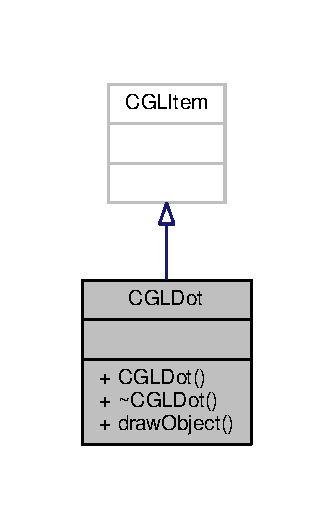
\includegraphics[width=160pt]{d3/d95/class_c_g_l_dot__inherit__graph}
\end{center}
\end{figure}


Graphe de collaboration de C\-G\-L\-Dot\-:
\nopagebreak
\begin{figure}[H]
\begin{center}
\leavevmode
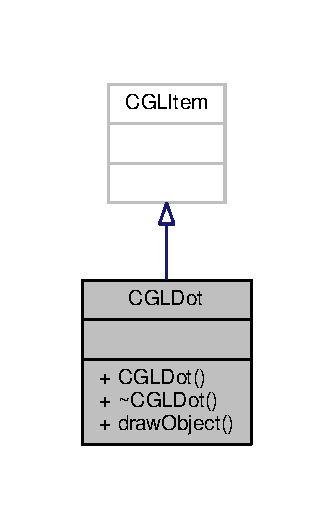
\includegraphics[width=160pt]{d7/d23/class_c_g_l_dot__coll__graph}
\end{center}
\end{figure}
\subsection*{Fonctions membres publiques}
\begin{DoxyCompactItemize}
\item 
\hyperlink{class_c_g_l_dot_a2199cd6c78e18219c88bf707201b003c}{C\-G\-L\-Dot} ()
\item 
virtual \hyperlink{class_c_g_l_dot_a9874d2a0168a7d8489c1bb7a6d6dc02c}{$\sim$\-C\-G\-L\-Dot} ()
\item 
void \hyperlink{class_c_g_l_dot_aba6d02d4c9da30aea263599e66e5f201}{draw\-Object} (Uint32 ellapsed\-Time)
\end{DoxyCompactItemize}


\subsection{Description détaillée}


Définition à la ligne 16 du fichier Dot.\-h.



\subsection{Documentation des constructeurs et destructeur}
\hypertarget{class_c_g_l_dot_a2199cd6c78e18219c88bf707201b003c}{\index{C\-G\-L\-Dot@{C\-G\-L\-Dot}!C\-G\-L\-Dot@{C\-G\-L\-Dot}}
\index{C\-G\-L\-Dot@{C\-G\-L\-Dot}!CGLDot@{C\-G\-L\-Dot}}
\subsubsection[{C\-G\-L\-Dot}]{\setlength{\rightskip}{0pt plus 5cm}C\-G\-L\-Dot\-::\-C\-G\-L\-Dot (
\begin{DoxyParamCaption}
{}
\end{DoxyParamCaption}
)}}\label{class_c_g_l_dot_a2199cd6c78e18219c88bf707201b003c}


Définition à la ligne 10 du fichier Dot.\-cpp.

\hypertarget{class_c_g_l_dot_a9874d2a0168a7d8489c1bb7a6d6dc02c}{\index{C\-G\-L\-Dot@{C\-G\-L\-Dot}!$\sim$\-C\-G\-L\-Dot@{$\sim$\-C\-G\-L\-Dot}}
\index{$\sim$\-C\-G\-L\-Dot@{$\sim$\-C\-G\-L\-Dot}!CGLDot@{C\-G\-L\-Dot}}
\subsubsection[{$\sim$\-C\-G\-L\-Dot}]{\setlength{\rightskip}{0pt plus 5cm}C\-G\-L\-Dot\-::$\sim$\-C\-G\-L\-Dot (
\begin{DoxyParamCaption}
{}
\end{DoxyParamCaption}
)\hspace{0.3cm}{\ttfamily [virtual]}}}\label{class_c_g_l_dot_a9874d2a0168a7d8489c1bb7a6d6dc02c}


Définition à la ligne 14 du fichier Dot.\-cpp.



\subsection{Documentation des fonctions membres}
\hypertarget{class_c_g_l_dot_aba6d02d4c9da30aea263599e66e5f201}{\index{C\-G\-L\-Dot@{C\-G\-L\-Dot}!draw\-Object@{draw\-Object}}
\index{draw\-Object@{draw\-Object}!CGLDot@{C\-G\-L\-Dot}}
\subsubsection[{draw\-Object}]{\setlength{\rightskip}{0pt plus 5cm}void C\-G\-L\-Dot\-::draw\-Object (
\begin{DoxyParamCaption}
\item[{Uint32}]{ellapsed\-Time}
\end{DoxyParamCaption}
)}}\label{class_c_g_l_dot_aba6d02d4c9da30aea263599e66e5f201}


Définition à la ligne 18 du fichier Dot.\-cpp.



La documentation de cette classe a été générée à partir des fichiers suivants \-:\begin{DoxyCompactItemize}
\item 
/home/dagal/git/\-D\-G\-L/\-Damier\-G\-L/src/\-C\-G\-L/\hyperlink{_dot_8h}{Dot.\-h}\item 
/home/dagal/git/\-D\-G\-L/\-Damier\-G\-L/src/\-C\-G\-L/\hyperlink{_dot_8cpp}{Dot.\-cpp}\end{DoxyCompactItemize}

\hypertarget{class_c_g_l_line}{\section{Référence de la classe C\-G\-L\-Line}
\label{class_c_g_l_line}\index{C\-G\-L\-Line@{C\-G\-L\-Line}}
}


{\ttfamily \#include $<$Line.\-h$>$}



Graphe d'héritage de C\-G\-L\-Line\-:
\nopagebreak
\begin{figure}[H]
\begin{center}
\leavevmode
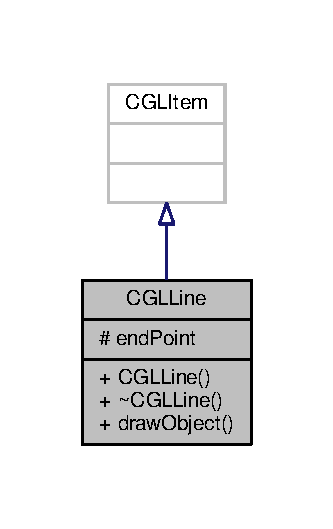
\includegraphics[width=160pt]{d9/dd7/class_c_g_l_line__inherit__graph}
\end{center}
\end{figure}


Graphe de collaboration de C\-G\-L\-Line\-:
\nopagebreak
\begin{figure}[H]
\begin{center}
\leavevmode
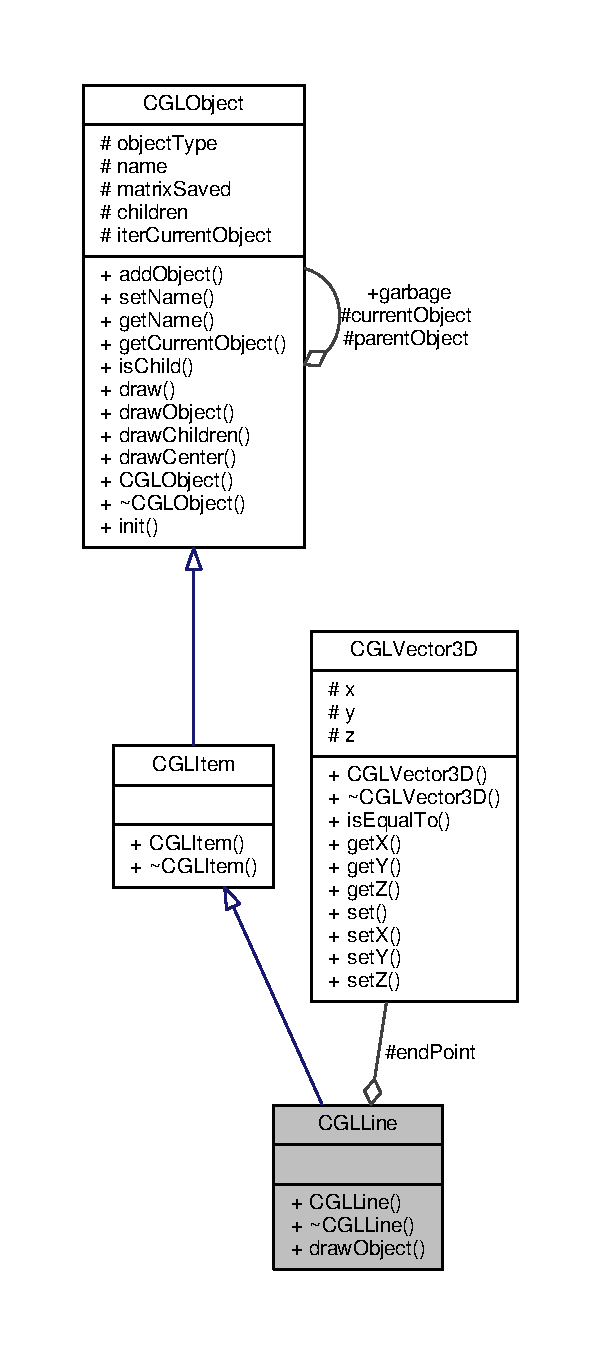
\includegraphics[width=160pt]{db/d95/class_c_g_l_line__coll__graph}
\end{center}
\end{figure}
\subsection*{Fonctions membres publiques}
\begin{DoxyCompactItemize}
\item 
\hyperlink{class_c_g_l_line_ab220112ce9d381cc057e6cff09fd95a7}{C\-G\-L\-Line} ()
\item 
virtual \hyperlink{class_c_g_l_line_ae00c52a8b8890cbe7657862aad150022}{$\sim$\-C\-G\-L\-Line} ()
\item 
void \hyperlink{class_c_g_l_line_a9621fa37a8b87f06e2a67aa8bf17d957}{draw\-Object} (Uint32 ellapsed\-Time)
\end{DoxyCompactItemize}
\subsection*{Attributs protégés}
\begin{DoxyCompactItemize}
\item 
C\-G\-L\-Vector3\-D \hyperlink{class_c_g_l_line_a2c4e6d2079bbac662dddf3fc137ad4d9}{end\-Point}
\end{DoxyCompactItemize}


\subsection{Description détaillée}


Définition à la ligne 17 du fichier Line.\-h.



\subsection{Documentation des constructeurs et destructeur}
\hypertarget{class_c_g_l_line_ab220112ce9d381cc057e6cff09fd95a7}{\index{C\-G\-L\-Line@{C\-G\-L\-Line}!C\-G\-L\-Line@{C\-G\-L\-Line}}
\index{C\-G\-L\-Line@{C\-G\-L\-Line}!CGLLine@{C\-G\-L\-Line}}
\subsubsection[{C\-G\-L\-Line}]{\setlength{\rightskip}{0pt plus 5cm}C\-G\-L\-Line\-::\-C\-G\-L\-Line (
\begin{DoxyParamCaption}
{}
\end{DoxyParamCaption}
)}}\label{class_c_g_l_line_ab220112ce9d381cc057e6cff09fd95a7}


Définition à la ligne 10 du fichier Line.\-cpp.

\hypertarget{class_c_g_l_line_ae00c52a8b8890cbe7657862aad150022}{\index{C\-G\-L\-Line@{C\-G\-L\-Line}!$\sim$\-C\-G\-L\-Line@{$\sim$\-C\-G\-L\-Line}}
\index{$\sim$\-C\-G\-L\-Line@{$\sim$\-C\-G\-L\-Line}!CGLLine@{C\-G\-L\-Line}}
\subsubsection[{$\sim$\-C\-G\-L\-Line}]{\setlength{\rightskip}{0pt plus 5cm}C\-G\-L\-Line\-::$\sim$\-C\-G\-L\-Line (
\begin{DoxyParamCaption}
{}
\end{DoxyParamCaption}
)\hspace{0.3cm}{\ttfamily [virtual]}}}\label{class_c_g_l_line_ae00c52a8b8890cbe7657862aad150022}


Définition à la ligne 15 du fichier Line.\-cpp.



\subsection{Documentation des fonctions membres}
\hypertarget{class_c_g_l_line_a9621fa37a8b87f06e2a67aa8bf17d957}{\index{C\-G\-L\-Line@{C\-G\-L\-Line}!draw\-Object@{draw\-Object}}
\index{draw\-Object@{draw\-Object}!CGLLine@{C\-G\-L\-Line}}
\subsubsection[{draw\-Object}]{\setlength{\rightskip}{0pt plus 5cm}void C\-G\-L\-Line\-::draw\-Object (
\begin{DoxyParamCaption}
\item[{Uint32}]{ellapsed\-Time}
\end{DoxyParamCaption}
)}}\label{class_c_g_l_line_a9621fa37a8b87f06e2a67aa8bf17d957}


Définition à la ligne 19 du fichier Line.\-cpp.



\subsection{Documentation des données membres}
\hypertarget{class_c_g_l_line_a2c4e6d2079bbac662dddf3fc137ad4d9}{\index{C\-G\-L\-Line@{C\-G\-L\-Line}!end\-Point@{end\-Point}}
\index{end\-Point@{end\-Point}!CGLLine@{C\-G\-L\-Line}}
\subsubsection[{end\-Point}]{\setlength{\rightskip}{0pt plus 5cm}C\-G\-L\-Vector3\-D C\-G\-L\-Line\-::end\-Point\hspace{0.3cm}{\ttfamily [protected]}}}\label{class_c_g_l_line_a2c4e6d2079bbac662dddf3fc137ad4d9}


Définition à la ligne 20 du fichier Line.\-h.



La documentation de cette classe a été générée à partir des fichiers suivants \-:\begin{DoxyCompactItemize}
\item 
/home/dagal/git/\-D\-G\-L/\-Damier\-G\-L/src/\-C\-G\-L/\hyperlink{_line_8h}{Line.\-h}\item 
/home/dagal/git/\-D\-G\-L/\-Damier\-G\-L/src/\-C\-G\-L/\hyperlink{_line_8cpp}{Line.\-cpp}\end{DoxyCompactItemize}

\hypertarget{class_c_g_l_polygon}{\section{Référence de la classe C\-G\-L\-Polygon}
\label{class_c_g_l_polygon}\index{C\-G\-L\-Polygon@{C\-G\-L\-Polygon}}
}


{\ttfamily \#include $<$Polygon.\-h$>$}



Graphe d'héritage de C\-G\-L\-Polygon\-:
\nopagebreak
\begin{figure}[H]
\begin{center}
\leavevmode
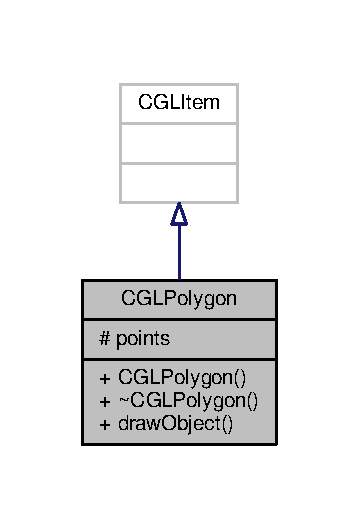
\includegraphics[width=172pt]{d9/d48/class_c_g_l_polygon__inherit__graph}
\end{center}
\end{figure}


Graphe de collaboration de C\-G\-L\-Polygon\-:
\nopagebreak
\begin{figure}[H]
\begin{center}
\leavevmode
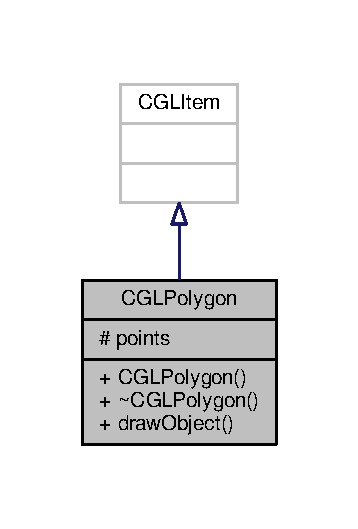
\includegraphics[width=172pt]{d0/d36/class_c_g_l_polygon__coll__graph}
\end{center}
\end{figure}
\subsection*{Fonctions membres publiques}
\begin{DoxyCompactItemize}
\item 
\hyperlink{class_c_g_l_polygon_a7727830b4fa06ad9d4fdd684d03525ab}{C\-G\-L\-Polygon} ()
\item 
virtual \hyperlink{class_c_g_l_polygon_a87b29787eaf2def21bcc61cf5cd0d76c}{$\sim$\-C\-G\-L\-Polygon} ()
\item 
void \hyperlink{class_c_g_l_polygon_a8450b134d7e40059c36ecc43133596c0}{draw\-Object} (Uint32 ellapsed\-Time)
\end{DoxyCompactItemize}
\subsection*{Attributs protégés}
\begin{DoxyCompactItemize}
\item 
list$<$ \hyperlink{class_c_g_l_vector2_d}{C\-G\-L\-Vector2\-D} $\ast$ $>$ \hyperlink{class_c_g_l_polygon_a8092f33a46cc4b79554808efa24ba025}{points}
\end{DoxyCompactItemize}


\subsection{Description détaillée}


Définition à la ligne 20 du fichier Polygon.\-h.



\subsection{Documentation des constructeurs et destructeur}
\hypertarget{class_c_g_l_polygon_a7727830b4fa06ad9d4fdd684d03525ab}{\index{C\-G\-L\-Polygon@{C\-G\-L\-Polygon}!C\-G\-L\-Polygon@{C\-G\-L\-Polygon}}
\index{C\-G\-L\-Polygon@{C\-G\-L\-Polygon}!CGLPolygon@{C\-G\-L\-Polygon}}
\subsubsection[{C\-G\-L\-Polygon}]{\setlength{\rightskip}{0pt plus 5cm}C\-G\-L\-Polygon\-::\-C\-G\-L\-Polygon (
\begin{DoxyParamCaption}
{}
\end{DoxyParamCaption}
)}}\label{class_c_g_l_polygon_a7727830b4fa06ad9d4fdd684d03525ab}


Définition à la ligne 10 du fichier Polygon.\-cpp.

\hypertarget{class_c_g_l_polygon_a87b29787eaf2def21bcc61cf5cd0d76c}{\index{C\-G\-L\-Polygon@{C\-G\-L\-Polygon}!$\sim$\-C\-G\-L\-Polygon@{$\sim$\-C\-G\-L\-Polygon}}
\index{$\sim$\-C\-G\-L\-Polygon@{$\sim$\-C\-G\-L\-Polygon}!CGLPolygon@{C\-G\-L\-Polygon}}
\subsubsection[{$\sim$\-C\-G\-L\-Polygon}]{\setlength{\rightskip}{0pt plus 5cm}C\-G\-L\-Polygon\-::$\sim$\-C\-G\-L\-Polygon (
\begin{DoxyParamCaption}
{}
\end{DoxyParamCaption}
)\hspace{0.3cm}{\ttfamily [virtual]}}}\label{class_c_g_l_polygon_a87b29787eaf2def21bcc61cf5cd0d76c}


Définition à la ligne 24 du fichier Polygon.\-cpp.



\subsection{Documentation des fonctions membres}
\hypertarget{class_c_g_l_polygon_a8450b134d7e40059c36ecc43133596c0}{\index{C\-G\-L\-Polygon@{C\-G\-L\-Polygon}!draw\-Object@{draw\-Object}}
\index{draw\-Object@{draw\-Object}!CGLPolygon@{C\-G\-L\-Polygon}}
\subsubsection[{draw\-Object}]{\setlength{\rightskip}{0pt plus 5cm}void C\-G\-L\-Polygon\-::draw\-Object (
\begin{DoxyParamCaption}
\item[{Uint32}]{ellapsed\-Time}
\end{DoxyParamCaption}
)}}\label{class_c_g_l_polygon_a8450b134d7e40059c36ecc43133596c0}


Définition à la ligne 29 du fichier Polygon.\-cpp.



\subsection{Documentation des données membres}
\hypertarget{class_c_g_l_polygon_a8092f33a46cc4b79554808efa24ba025}{\index{C\-G\-L\-Polygon@{C\-G\-L\-Polygon}!points@{points}}
\index{points@{points}!CGLPolygon@{C\-G\-L\-Polygon}}
\subsubsection[{points}]{\setlength{\rightskip}{0pt plus 5cm}list$<${\bf C\-G\-L\-Vector2\-D}$\ast$$>$ C\-G\-L\-Polygon\-::points\hspace{0.3cm}{\ttfamily [protected]}}}\label{class_c_g_l_polygon_a8092f33a46cc4b79554808efa24ba025}


Définition à la ligne 23 du fichier Polygon.\-h.



La documentation de cette classe a été générée à partir des fichiers suivants \-:\begin{DoxyCompactItemize}
\item 
/home/dagal/git/\-D\-G\-L/\-Damier\-G\-L/src/\-C\-G\-L/\hyperlink{_polygon_8h}{Polygon.\-h}\item 
/home/dagal/git/\-D\-G\-L/\-Damier\-G\-L/src/\-C\-G\-L/\hyperlink{_polygon_8cpp}{Polygon.\-cpp}\end{DoxyCompactItemize}

\hypertarget{class_c_g_l_position}{\section{Référence de la classe C\-G\-L\-Position}
\label{class_c_g_l_position}\index{C\-G\-L\-Position@{C\-G\-L\-Position}}
}


{\ttfamily \#include $<$Position.\-h$>$}



Graphe d'héritage de C\-G\-L\-Position\-:
\nopagebreak
\begin{figure}[H]
\begin{center}
\leavevmode
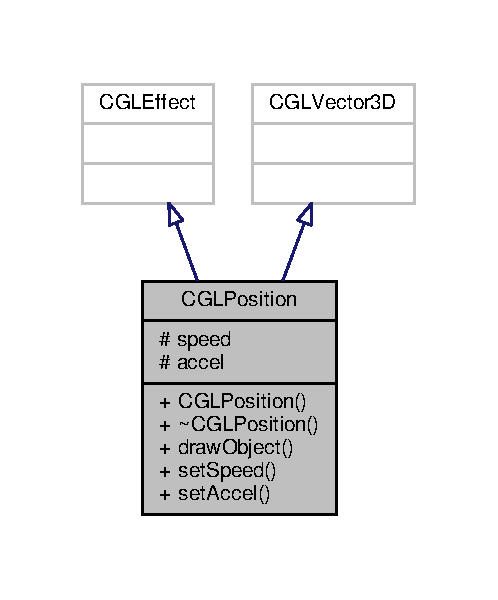
\includegraphics[width=239pt]{d7/d46/class_c_g_l_position__inherit__graph}
\end{center}
\end{figure}


Graphe de collaboration de C\-G\-L\-Position\-:
\nopagebreak
\begin{figure}[H]
\begin{center}
\leavevmode
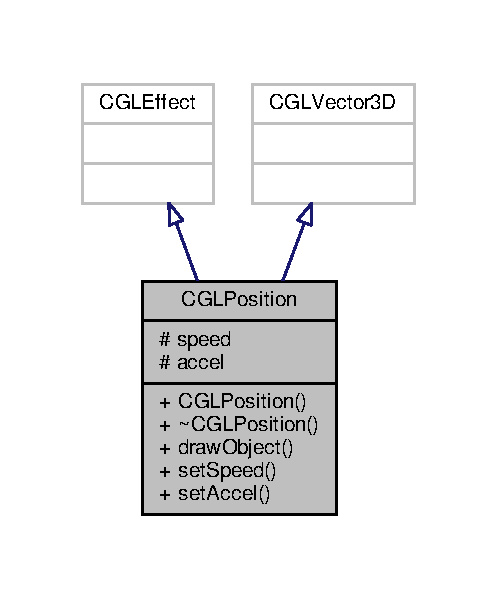
\includegraphics[width=239pt]{df/df1/class_c_g_l_position__coll__graph}
\end{center}
\end{figure}
\subsection*{Fonctions membres publiques}
\begin{DoxyCompactItemize}
\item 
\hyperlink{class_c_g_l_position_ab32bdd49fc31414e874917568e5d37d2}{C\-G\-L\-Position} ()
\item 
virtual \hyperlink{class_c_g_l_position_afe1ee045b528494d23286adf06aecae0}{$\sim$\-C\-G\-L\-Position} ()
\item 
void \hyperlink{class_c_g_l_position_a439ae873ba7ef56826a27eb7b15b0b6f}{draw\-Object} (Uint32 ellapsed\-Time)
\item 
void \hyperlink{class_c_g_l_position_a729e7b3f01b8c735d60d8c51b6610eef}{set\-Speed} (double const sx, double const sy, double const sz)
\item 
void \hyperlink{class_c_g_l_position_a5a43a8991d3d8ca645edbcfb0e97db20}{set\-Accel} (double const ax, double const ay, double const az)
\end{DoxyCompactItemize}
\subsection*{Attributs protégés}
\begin{DoxyCompactItemize}
\item 
C\-G\-L\-Vector3\-D \hyperlink{class_c_g_l_position_ac5a3b64ac5c800b84a3b621e6e50c381}{speed}
\item 
C\-G\-L\-Vector3\-D \hyperlink{class_c_g_l_position_abb7ae2f19acbbcc53d685c9ee0e948ce}{accel}
\end{DoxyCompactItemize}


\subsection{Description détaillée}


Définition à la ligne 14 du fichier Position.\-h.



\subsection{Documentation des constructeurs et destructeur}
\hypertarget{class_c_g_l_position_ab32bdd49fc31414e874917568e5d37d2}{\index{C\-G\-L\-Position@{C\-G\-L\-Position}!C\-G\-L\-Position@{C\-G\-L\-Position}}
\index{C\-G\-L\-Position@{C\-G\-L\-Position}!CGLPosition@{C\-G\-L\-Position}}
\subsubsection[{C\-G\-L\-Position}]{\setlength{\rightskip}{0pt plus 5cm}C\-G\-L\-Position\-::\-C\-G\-L\-Position (
\begin{DoxyParamCaption}
{}
\end{DoxyParamCaption}
)}}\label{class_c_g_l_position_ab32bdd49fc31414e874917568e5d37d2}


Définition à la ligne 10 du fichier Position.\-cpp.

\hypertarget{class_c_g_l_position_afe1ee045b528494d23286adf06aecae0}{\index{C\-G\-L\-Position@{C\-G\-L\-Position}!$\sim$\-C\-G\-L\-Position@{$\sim$\-C\-G\-L\-Position}}
\index{$\sim$\-C\-G\-L\-Position@{$\sim$\-C\-G\-L\-Position}!CGLPosition@{C\-G\-L\-Position}}
\subsubsection[{$\sim$\-C\-G\-L\-Position}]{\setlength{\rightskip}{0pt plus 5cm}C\-G\-L\-Position\-::$\sim$\-C\-G\-L\-Position (
\begin{DoxyParamCaption}
{}
\end{DoxyParamCaption}
)\hspace{0.3cm}{\ttfamily [virtual]}}}\label{class_c_g_l_position_afe1ee045b528494d23286adf06aecae0}


Définition à la ligne 16 du fichier Position.\-cpp.



\subsection{Documentation des fonctions membres}
\hypertarget{class_c_g_l_position_a439ae873ba7ef56826a27eb7b15b0b6f}{\index{C\-G\-L\-Position@{C\-G\-L\-Position}!draw\-Object@{draw\-Object}}
\index{draw\-Object@{draw\-Object}!CGLPosition@{C\-G\-L\-Position}}
\subsubsection[{draw\-Object}]{\setlength{\rightskip}{0pt plus 5cm}void C\-G\-L\-Position\-::draw\-Object (
\begin{DoxyParamCaption}
\item[{Uint32}]{ellapsed\-Time}
\end{DoxyParamCaption}
)}}\label{class_c_g_l_position_a439ae873ba7ef56826a27eb7b15b0b6f}


Définition à la ligne 30 du fichier Position.\-cpp.

\hypertarget{class_c_g_l_position_a5a43a8991d3d8ca645edbcfb0e97db20}{\index{C\-G\-L\-Position@{C\-G\-L\-Position}!set\-Accel@{set\-Accel}}
\index{set\-Accel@{set\-Accel}!CGLPosition@{C\-G\-L\-Position}}
\subsubsection[{set\-Accel}]{\setlength{\rightskip}{0pt plus 5cm}void C\-G\-L\-Position\-::set\-Accel (
\begin{DoxyParamCaption}
\item[{double const}]{ax, }
\item[{double const}]{ay, }
\item[{double const}]{az}
\end{DoxyParamCaption}
)}}\label{class_c_g_l_position_a5a43a8991d3d8ca645edbcfb0e97db20}


Définition à la ligne 25 du fichier Position.\-cpp.



Voici le graphe des appelants de cette fonction \-:
\nopagebreak
\begin{figure}[H]
\begin{center}
\leavevmode
\includegraphics[width=270pt]{de/d31/class_c_g_l_position_a5a43a8991d3d8ca645edbcfb0e97db20_icgraph}
\end{center}
\end{figure}


\hypertarget{class_c_g_l_position_a729e7b3f01b8c735d60d8c51b6610eef}{\index{C\-G\-L\-Position@{C\-G\-L\-Position}!set\-Speed@{set\-Speed}}
\index{set\-Speed@{set\-Speed}!CGLPosition@{C\-G\-L\-Position}}
\subsubsection[{set\-Speed}]{\setlength{\rightskip}{0pt plus 5cm}void C\-G\-L\-Position\-::set\-Speed (
\begin{DoxyParamCaption}
\item[{double const}]{sx, }
\item[{double const}]{sy, }
\item[{double const}]{sz}
\end{DoxyParamCaption}
)}}\label{class_c_g_l_position_a729e7b3f01b8c735d60d8c51b6610eef}


Définition à la ligne 20 du fichier Position.\-cpp.



Voici le graphe des appelants de cette fonction \-:
\nopagebreak
\begin{figure}[H]
\begin{center}
\leavevmode
\includegraphics[width=274pt]{de/d31/class_c_g_l_position_a729e7b3f01b8c735d60d8c51b6610eef_icgraph}
\end{center}
\end{figure}




\subsection{Documentation des données membres}
\hypertarget{class_c_g_l_position_abb7ae2f19acbbcc53d685c9ee0e948ce}{\index{C\-G\-L\-Position@{C\-G\-L\-Position}!accel@{accel}}
\index{accel@{accel}!CGLPosition@{C\-G\-L\-Position}}
\subsubsection[{accel}]{\setlength{\rightskip}{0pt plus 5cm}C\-G\-L\-Vector3\-D C\-G\-L\-Position\-::accel\hspace{0.3cm}{\ttfamily [protected]}}}\label{class_c_g_l_position_abb7ae2f19acbbcc53d685c9ee0e948ce}


Définition à la ligne 21 du fichier Position.\-h.

\hypertarget{class_c_g_l_position_ac5a3b64ac5c800b84a3b621e6e50c381}{\index{C\-G\-L\-Position@{C\-G\-L\-Position}!speed@{speed}}
\index{speed@{speed}!CGLPosition@{C\-G\-L\-Position}}
\subsubsection[{speed}]{\setlength{\rightskip}{0pt plus 5cm}C\-G\-L\-Vector3\-D C\-G\-L\-Position\-::speed\hspace{0.3cm}{\ttfamily [protected]}}}\label{class_c_g_l_position_ac5a3b64ac5c800b84a3b621e6e50c381}


Définition à la ligne 20 du fichier Position.\-h.



La documentation de cette classe a été générée à partir des fichiers suivants \-:\begin{DoxyCompactItemize}
\item 
/home/dagal/git/\-D\-G\-L/\-Damier\-G\-L/src/\-C\-G\-L/\hyperlink{_position_8h}{Position.\-h}\item 
/home/dagal/git/\-D\-G\-L/\-Damier\-G\-L/src/\-C\-G\-L/\hyperlink{_position_8cpp}{Position.\-cpp}\end{DoxyCompactItemize}

\hypertarget{class_c_g_l_quad}{\section{Référence de la classe C\-G\-L\-Quad}
\label{class_c_g_l_quad}\index{C\-G\-L\-Quad@{C\-G\-L\-Quad}}
}


{\ttfamily \#include $<$C\-G\-L\-Quad.\-h$>$}



Graphe d'héritage de C\-G\-L\-Quad\-:\nopagebreak
\begin{figure}[H]
\begin{center}
\leavevmode
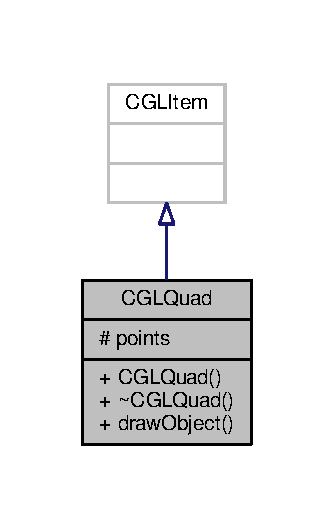
\includegraphics[height=550pt]{d8/de4/class_c_g_l_quad__inherit__graph}
\end{center}
\end{figure}


Graphe de collaboration de C\-G\-L\-Quad\-:\nopagebreak
\begin{figure}[H]
\begin{center}
\leavevmode
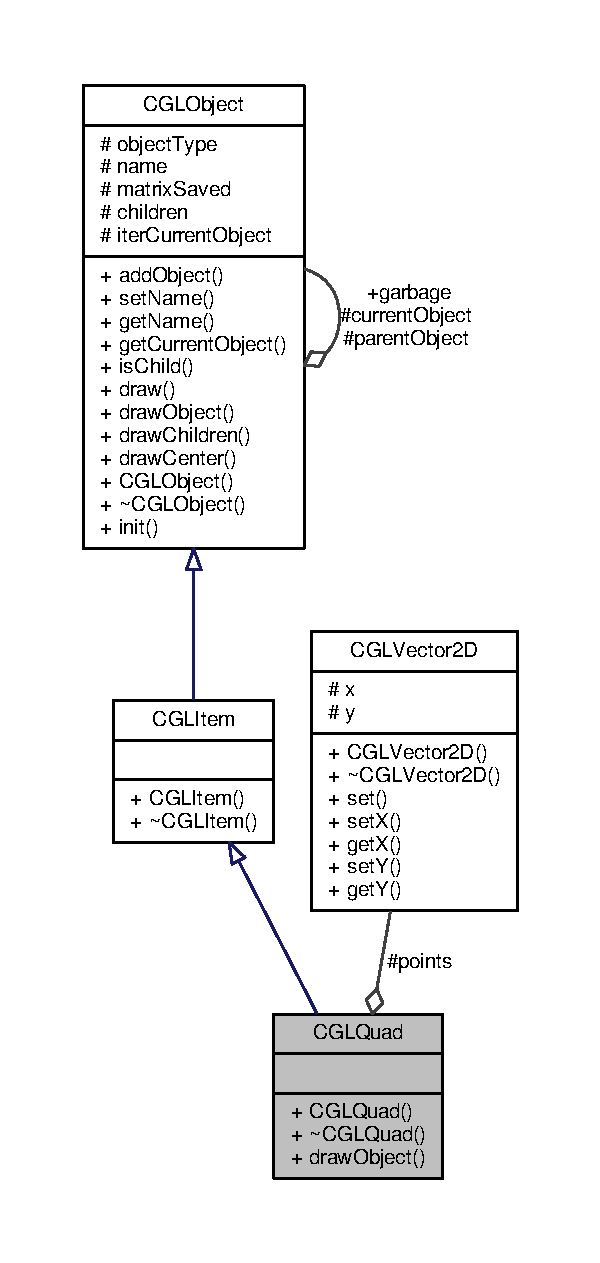
\includegraphics[width=267pt]{dd/d46/class_c_g_l_quad__coll__graph}
\end{center}
\end{figure}
\subsection*{Fonctions membres publiques}
\begin{DoxyCompactItemize}
\item 
\hyperlink{class_c_g_l_quad_a95b07c1605f65de30cb47b65fa364294}{C\-G\-L\-Quad} ()
\item 
\hyperlink{class_c_g_l_quad_a6a78f1183a166adf08bfe3880f2cd415}{C\-G\-L\-Quad} (double x, double y, double z, double r)
\item 
virtual \hyperlink{class_c_g_l_quad_a19320cf64816de2de1fa7540acbf833e}{$\sim$\-C\-G\-L\-Quad} ()
\item 
void \hyperlink{class_c_g_l_quad_a81696d558e2355af7d621cdbf0ccf41a}{draw\-Object} (Uint32 time\-Ellapsed)
\end{DoxyCompactItemize}
\subsection*{Attributs protégés}
\begin{DoxyCompactItemize}
\item 
double \hyperlink{class_c_g_l_quad_a53dcf6352ff92cde8cc4b9756e51057e}{longueur}
\end{DoxyCompactItemize}
\subsection*{Membres hérités additionnels}


\subsection{Description détaillée}


Définition à la ligne 13 du fichier C\-G\-L\-Quad.\-h.



\subsection{Documentation des constructeurs et destructeur}
\hypertarget{class_c_g_l_quad_a95b07c1605f65de30cb47b65fa364294}{\index{C\-G\-L\-Quad@{C\-G\-L\-Quad}!C\-G\-L\-Quad@{C\-G\-L\-Quad}}
\index{C\-G\-L\-Quad@{C\-G\-L\-Quad}!CGLQuad@{C\-G\-L\-Quad}}
\subsubsection[{C\-G\-L\-Quad}]{\setlength{\rightskip}{0pt plus 5cm}C\-G\-L\-Quad\-::\-C\-G\-L\-Quad (
\begin{DoxyParamCaption}
{}
\end{DoxyParamCaption}
)}}\label{class_c_g_l_quad_a95b07c1605f65de30cb47b65fa364294}


Définition à la ligne 10 du fichier C\-G\-L\-Quad.\-cpp.

\hypertarget{class_c_g_l_quad_a6a78f1183a166adf08bfe3880f2cd415}{\index{C\-G\-L\-Quad@{C\-G\-L\-Quad}!C\-G\-L\-Quad@{C\-G\-L\-Quad}}
\index{C\-G\-L\-Quad@{C\-G\-L\-Quad}!CGLQuad@{C\-G\-L\-Quad}}
\subsubsection[{C\-G\-L\-Quad}]{\setlength{\rightskip}{0pt plus 5cm}C\-G\-L\-Quad\-::\-C\-G\-L\-Quad (
\begin{DoxyParamCaption}
\item[{double}]{x, }
\item[{double}]{y, }
\item[{double}]{z, }
\item[{double}]{r}
\end{DoxyParamCaption}
)}}\label{class_c_g_l_quad_a6a78f1183a166adf08bfe3880f2cd415}


Définition à la ligne 16 du fichier C\-G\-L\-Quad.\-cpp.

\hypertarget{class_c_g_l_quad_a19320cf64816de2de1fa7540acbf833e}{\index{C\-G\-L\-Quad@{C\-G\-L\-Quad}!$\sim$\-C\-G\-L\-Quad@{$\sim$\-C\-G\-L\-Quad}}
\index{$\sim$\-C\-G\-L\-Quad@{$\sim$\-C\-G\-L\-Quad}!CGLQuad@{C\-G\-L\-Quad}}
\subsubsection[{$\sim$\-C\-G\-L\-Quad}]{\setlength{\rightskip}{0pt plus 5cm}C\-G\-L\-Quad\-::$\sim$\-C\-G\-L\-Quad (
\begin{DoxyParamCaption}
{}
\end{DoxyParamCaption}
)\hspace{0.3cm}{\ttfamily [virtual]}}}\label{class_c_g_l_quad_a19320cf64816de2de1fa7540acbf833e}


Définition à la ligne 21 du fichier C\-G\-L\-Quad.\-cpp.



\subsection{Documentation des fonctions membres}
\hypertarget{class_c_g_l_quad_a81696d558e2355af7d621cdbf0ccf41a}{\index{C\-G\-L\-Quad@{C\-G\-L\-Quad}!draw\-Object@{draw\-Object}}
\index{draw\-Object@{draw\-Object}!CGLQuad@{C\-G\-L\-Quad}}
\subsubsection[{draw\-Object}]{\setlength{\rightskip}{0pt plus 5cm}void C\-G\-L\-Quad\-::draw\-Object (
\begin{DoxyParamCaption}
\item[{Uint32}]{time\-Ellapsed}
\end{DoxyParamCaption}
)\hspace{0.3cm}{\ttfamily [virtual]}}}\label{class_c_g_l_quad_a81696d558e2355af7d621cdbf0ccf41a}


Réimplémentée à partir de \hyperlink{class_c_g_l_object_a2781ec98c37bd209f2382c5130a365b9}{C\-G\-L\-Object}.



Définition à la ligne 25 du fichier C\-G\-L\-Quad.\-cpp.



Voici le graphe d'appel pour cette fonction \-:\nopagebreak
\begin{figure}[H]
\begin{center}
\leavevmode
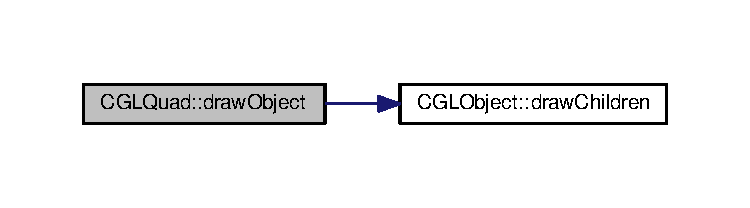
\includegraphics[width=350pt]{df/d41/class_c_g_l_quad_a81696d558e2355af7d621cdbf0ccf41a_cgraph}
\end{center}
\end{figure}




\subsection{Documentation des données membres}
\hypertarget{class_c_g_l_quad_a53dcf6352ff92cde8cc4b9756e51057e}{\index{C\-G\-L\-Quad@{C\-G\-L\-Quad}!longueur@{longueur}}
\index{longueur@{longueur}!CGLQuad@{C\-G\-L\-Quad}}
\subsubsection[{longueur}]{\setlength{\rightskip}{0pt plus 5cm}double C\-G\-L\-Quad\-::longueur\hspace{0.3cm}{\ttfamily [protected]}}}\label{class_c_g_l_quad_a53dcf6352ff92cde8cc4b9756e51057e}


Définition à la ligne 18 du fichier C\-G\-L\-Quad.\-h.



La documentation de cette classe a été générée à partir des fichiers suivants \-:\begin{DoxyCompactItemize}
\item 
/home/dagal/git/\-Damier\-G\-L/\-Damier\-G\-L/src/\-C\-G\-L/\hyperlink{_c_g_l_quad_8h}{C\-G\-L\-Quad.\-h}\item 
/home/dagal/git/\-Damier\-G\-L/\-Damier\-G\-L/src/\-C\-G\-L/\hyperlink{_c_g_l_quad_8cpp}{C\-G\-L\-Quad.\-cpp}\end{DoxyCompactItemize}

\hypertarget{class_c_g_l_robot1}{\section{Référence de la classe C\-G\-L\-Robot1}
\label{class_c_g_l_robot1}\index{C\-G\-L\-Robot1@{C\-G\-L\-Robot1}}
}


{\ttfamily \#include $<$Robot1.\-h$>$}



Graphe d'héritage de C\-G\-L\-Robot1\-:
\nopagebreak
\begin{figure}[H]
\begin{center}
\leavevmode
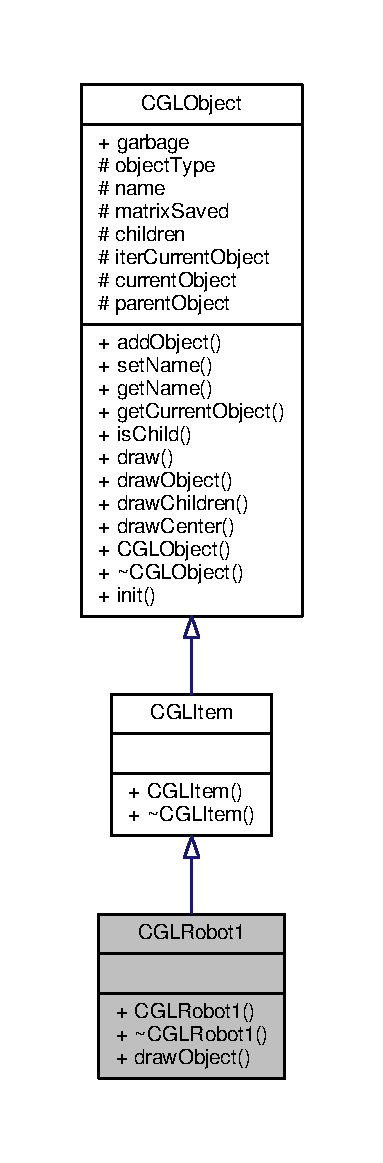
\includegraphics[width=168pt]{d2/dcc/class_c_g_l_robot1__inherit__graph}
\end{center}
\end{figure}


Graphe de collaboration de C\-G\-L\-Robot1\-:
\nopagebreak
\begin{figure}[H]
\begin{center}
\leavevmode
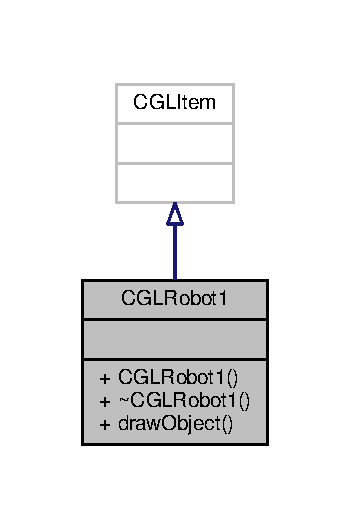
\includegraphics[width=168pt]{dc/de7/class_c_g_l_robot1__coll__graph}
\end{center}
\end{figure}
\subsection*{Fonctions membres publiques}
\begin{DoxyCompactItemize}
\item 
\hyperlink{class_c_g_l_robot1_a2b8077cc29b703e31d3ec85404cd3aed}{C\-G\-L\-Robot1} ()
\item 
virtual \hyperlink{class_c_g_l_robot1_accda840d084f72fb65d243dc047abc11}{$\sim$\-C\-G\-L\-Robot1} ()
\item 
void \hyperlink{class_c_g_l_robot1_a050d7fea4097a6634ef5feef26ae7865}{draw\-Object} (Uint32 time\-Ellapsed)
\end{DoxyCompactItemize}


\subsection{Description détaillée}


Définition à la ligne 13 du fichier Robot1.\-h.



\subsection{Documentation des constructeurs et destructeur}
\hypertarget{class_c_g_l_robot1_a2b8077cc29b703e31d3ec85404cd3aed}{\index{C\-G\-L\-Robot1@{C\-G\-L\-Robot1}!C\-G\-L\-Robot1@{C\-G\-L\-Robot1}}
\index{C\-G\-L\-Robot1@{C\-G\-L\-Robot1}!CGLRobot1@{C\-G\-L\-Robot1}}
\subsubsection[{C\-G\-L\-Robot1}]{\setlength{\rightskip}{0pt plus 5cm}C\-G\-L\-Robot1\-::\-C\-G\-L\-Robot1 (
\begin{DoxyParamCaption}
{}
\end{DoxyParamCaption}
)}}\label{class_c_g_l_robot1_a2b8077cc29b703e31d3ec85404cd3aed}


Définition à la ligne 10 du fichier Robot1.\-cpp.

\hypertarget{class_c_g_l_robot1_accda840d084f72fb65d243dc047abc11}{\index{C\-G\-L\-Robot1@{C\-G\-L\-Robot1}!$\sim$\-C\-G\-L\-Robot1@{$\sim$\-C\-G\-L\-Robot1}}
\index{$\sim$\-C\-G\-L\-Robot1@{$\sim$\-C\-G\-L\-Robot1}!CGLRobot1@{C\-G\-L\-Robot1}}
\subsubsection[{$\sim$\-C\-G\-L\-Robot1}]{\setlength{\rightskip}{0pt plus 5cm}C\-G\-L\-Robot1\-::$\sim$\-C\-G\-L\-Robot1 (
\begin{DoxyParamCaption}
{}
\end{DoxyParamCaption}
)\hspace{0.3cm}{\ttfamily [virtual]}}}\label{class_c_g_l_robot1_accda840d084f72fb65d243dc047abc11}


Définition à la ligne 26 du fichier Robot1.\-cpp.



\subsection{Documentation des fonctions membres}
\hypertarget{class_c_g_l_robot1_a050d7fea4097a6634ef5feef26ae7865}{\index{C\-G\-L\-Robot1@{C\-G\-L\-Robot1}!draw\-Object@{draw\-Object}}
\index{draw\-Object@{draw\-Object}!CGLRobot1@{C\-G\-L\-Robot1}}
\subsubsection[{draw\-Object}]{\setlength{\rightskip}{0pt plus 5cm}void C\-G\-L\-Robot1\-::draw\-Object (
\begin{DoxyParamCaption}
\item[{Uint32}]{time\-Ellapsed}
\end{DoxyParamCaption}
)}}\label{class_c_g_l_robot1_a050d7fea4097a6634ef5feef26ae7865}


Définition à la ligne 30 du fichier Robot1.\-cpp.



La documentation de cette classe a été générée à partir des fichiers suivants \-:\begin{DoxyCompactItemize}
\item 
/home/dagal/git/\-D\-G\-L/\-Damier\-G\-L/src/\-C\-G\-L/\hyperlink{_robot1_8h}{Robot1.\-h}\item 
/home/dagal/git/\-D\-G\-L/\-Damier\-G\-L/src/\-C\-G\-L/\hyperlink{_robot1_8cpp}{Robot1.\-cpp}\end{DoxyCompactItemize}

\hypertarget{class_c_g_l_rotation}{\section{Référence de la classe C\-G\-L\-Rotation}
\label{class_c_g_l_rotation}\index{C\-G\-L\-Rotation@{C\-G\-L\-Rotation}}
}


{\ttfamily \#include $<$C\-G\-L\-Rotation.\-h$>$}



Graphe d'héritage de C\-G\-L\-Rotation\-:\nopagebreak
\begin{figure}[H]
\begin{center}
\leavevmode
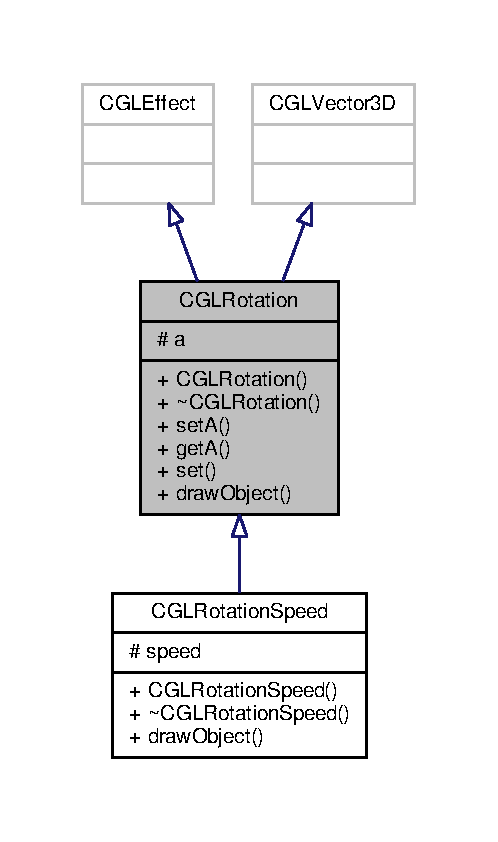
\includegraphics[height=550pt]{d4/d97/class_c_g_l_rotation__inherit__graph}
\end{center}
\end{figure}


Graphe de collaboration de C\-G\-L\-Rotation\-:\nopagebreak
\begin{figure}[H]
\begin{center}
\leavevmode
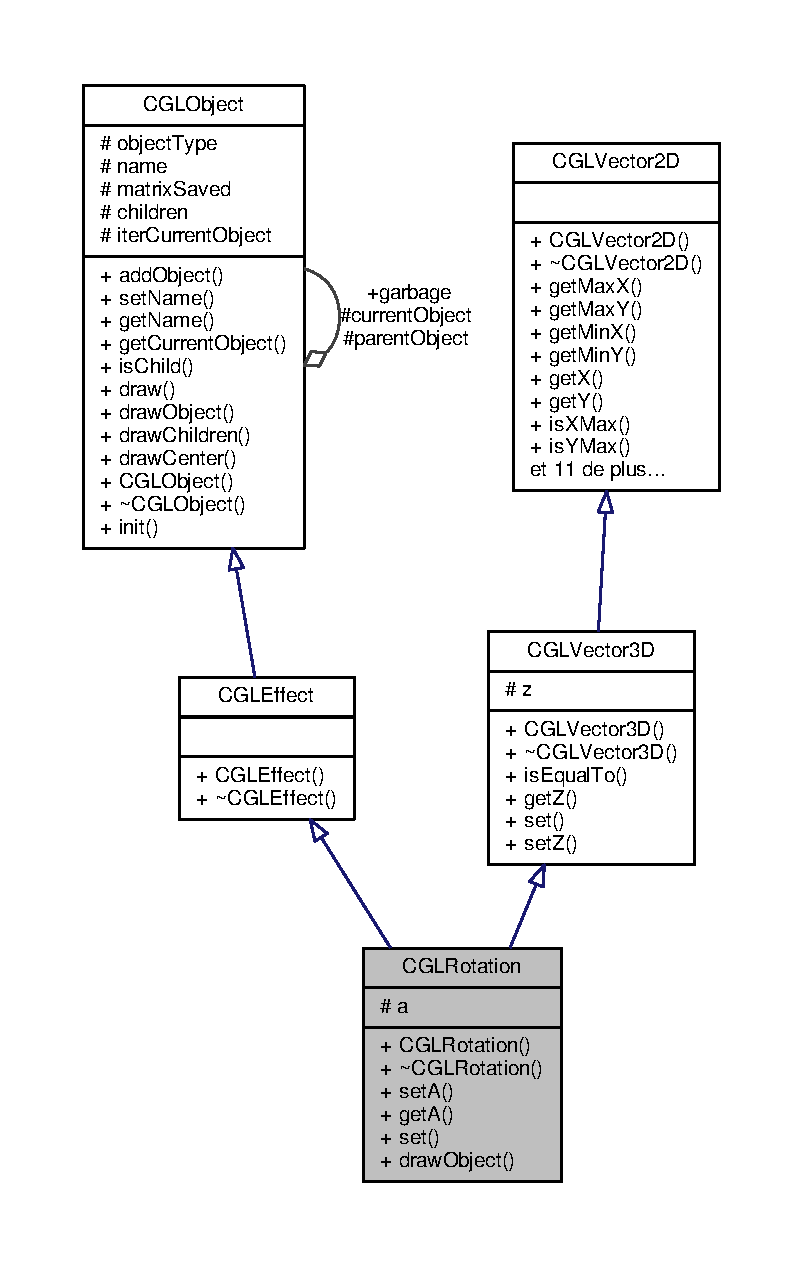
\includegraphics[height=550pt]{d0/db1/class_c_g_l_rotation__coll__graph}
\end{center}
\end{figure}
\subsection*{Fonctions membres publiques}
\begin{DoxyCompactItemize}
\item 
\hyperlink{class_c_g_l_rotation_a00f328e9aeefa148e4bd169afc5cb959}{C\-G\-L\-Rotation} ()
\item 
virtual \hyperlink{class_c_g_l_rotation_adc90213d4008b9beb3c8e266f952a509}{$\sim$\-C\-G\-L\-Rotation} ()
\item 
void \hyperlink{class_c_g_l_rotation_a690f30f8f121b27ac22d6b02a6443b58}{set\-A} (double av)
\item 
double \hyperlink{class_c_g_l_rotation_a0d836220b7b39ee00173ee4e0bb4da92}{get\-A} ()
\item 
void \hyperlink{class_c_g_l_rotation_a2b767e088f36ceef91e7259c76f7390e}{set} (double av, double ax, double ay, double az)
\item 
void \hyperlink{class_c_g_l_rotation_a94be2c089fbe52d0f8cb33ee98f8de74}{draw\-Object} (Uint32 ellapsed\-Time)
\end{DoxyCompactItemize}
\subsection*{Membres hérités additionnels}


\subsection{Description détaillée}


Définition à la ligne 17 du fichier C\-G\-L\-Rotation.\-h.



\subsection{Documentation des constructeurs et destructeur}
\hypertarget{class_c_g_l_rotation_a00f328e9aeefa148e4bd169afc5cb959}{\index{C\-G\-L\-Rotation@{C\-G\-L\-Rotation}!C\-G\-L\-Rotation@{C\-G\-L\-Rotation}}
\index{C\-G\-L\-Rotation@{C\-G\-L\-Rotation}!CGLRotation@{C\-G\-L\-Rotation}}
\subsubsection[{C\-G\-L\-Rotation}]{\setlength{\rightskip}{0pt plus 5cm}C\-G\-L\-Rotation\-::\-C\-G\-L\-Rotation (
\begin{DoxyParamCaption}
{}
\end{DoxyParamCaption}
)}}\label{class_c_g_l_rotation_a00f328e9aeefa148e4bd169afc5cb959}


Définition à la ligne 10 du fichier C\-G\-L\-Rotation.\-cpp.

\hypertarget{class_c_g_l_rotation_adc90213d4008b9beb3c8e266f952a509}{\index{C\-G\-L\-Rotation@{C\-G\-L\-Rotation}!$\sim$\-C\-G\-L\-Rotation@{$\sim$\-C\-G\-L\-Rotation}}
\index{$\sim$\-C\-G\-L\-Rotation@{$\sim$\-C\-G\-L\-Rotation}!CGLRotation@{C\-G\-L\-Rotation}}
\subsubsection[{$\sim$\-C\-G\-L\-Rotation}]{\setlength{\rightskip}{0pt plus 5cm}C\-G\-L\-Rotation\-::$\sim$\-C\-G\-L\-Rotation (
\begin{DoxyParamCaption}
{}
\end{DoxyParamCaption}
)\hspace{0.3cm}{\ttfamily [virtual]}}}\label{class_c_g_l_rotation_adc90213d4008b9beb3c8e266f952a509}


Définition à la ligne 16 du fichier C\-G\-L\-Rotation.\-cpp.



\subsection{Documentation des fonctions membres}
\hypertarget{class_c_g_l_rotation_a94be2c089fbe52d0f8cb33ee98f8de74}{\index{C\-G\-L\-Rotation@{C\-G\-L\-Rotation}!draw\-Object@{draw\-Object}}
\index{draw\-Object@{draw\-Object}!CGLRotation@{C\-G\-L\-Rotation}}
\subsubsection[{draw\-Object}]{\setlength{\rightskip}{0pt plus 5cm}void C\-G\-L\-Rotation\-::draw\-Object (
\begin{DoxyParamCaption}
\item[{Uint32}]{ellapsed\-Time}
\end{DoxyParamCaption}
)\hspace{0.3cm}{\ttfamily [virtual]}}}\label{class_c_g_l_rotation_a94be2c089fbe52d0f8cb33ee98f8de74}


Réimplémentée à partir de \hyperlink{class_c_g_l_object_a2781ec98c37bd209f2382c5130a365b9}{C\-G\-L\-Object}.



Définition à la ligne 38 du fichier C\-G\-L\-Rotation.\-cpp.

\hypertarget{class_c_g_l_rotation_a0d836220b7b39ee00173ee4e0bb4da92}{\index{C\-G\-L\-Rotation@{C\-G\-L\-Rotation}!get\-A@{get\-A}}
\index{get\-A@{get\-A}!CGLRotation@{C\-G\-L\-Rotation}}
\subsubsection[{get\-A}]{\setlength{\rightskip}{0pt plus 5cm}double C\-G\-L\-Rotation\-::get\-A (
\begin{DoxyParamCaption}
{}
\end{DoxyParamCaption}
)}}\label{class_c_g_l_rotation_a0d836220b7b39ee00173ee4e0bb4da92}


Définition à la ligne 25 du fichier C\-G\-L\-Rotation.\-cpp.

\hypertarget{class_c_g_l_rotation_a2b767e088f36ceef91e7259c76f7390e}{\index{C\-G\-L\-Rotation@{C\-G\-L\-Rotation}!set@{set}}
\index{set@{set}!CGLRotation@{C\-G\-L\-Rotation}}
\subsubsection[{set}]{\setlength{\rightskip}{0pt plus 5cm}void C\-G\-L\-Rotation\-::set (
\begin{DoxyParamCaption}
\item[{double}]{av, }
\item[{double}]{ax, }
\item[{double}]{ay, }
\item[{double}]{az}
\end{DoxyParamCaption}
)}}\label{class_c_g_l_rotation_a2b767e088f36ceef91e7259c76f7390e}


Définition à la ligne 30 du fichier C\-G\-L\-Rotation.\-cpp.



Voici le graphe des appelants de cette fonction \-:\nopagebreak
\begin{figure}[H]
\begin{center}
\leavevmode
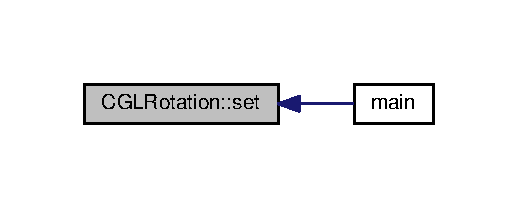
\includegraphics[width=248pt]{d4/dd5/class_c_g_l_rotation_a2b767e088f36ceef91e7259c76f7390e_icgraph}
\end{center}
\end{figure}


\hypertarget{class_c_g_l_rotation_a690f30f8f121b27ac22d6b02a6443b58}{\index{C\-G\-L\-Rotation@{C\-G\-L\-Rotation}!set\-A@{set\-A}}
\index{set\-A@{set\-A}!CGLRotation@{C\-G\-L\-Rotation}}
\subsubsection[{set\-A}]{\setlength{\rightskip}{0pt plus 5cm}void C\-G\-L\-Rotation\-::set\-A (
\begin{DoxyParamCaption}
\item[{double}]{av}
\end{DoxyParamCaption}
)}}\label{class_c_g_l_rotation_a690f30f8f121b27ac22d6b02a6443b58}


Définition à la ligne 20 du fichier C\-G\-L\-Rotation.\-cpp.



La documentation de cette classe a été générée à partir des fichiers suivants \-:\begin{DoxyCompactItemize}
\item 
/home/dagal/git/\-Damier\-G\-L/\-Damier\-G\-L/src/\-C\-G\-L/\hyperlink{_c_g_l_rotation_8h}{C\-G\-L\-Rotation.\-h}\item 
/home/dagal/git/\-Damier\-G\-L/\-Damier\-G\-L/src/\-C\-G\-L/\hyperlink{_c_g_l_rotation_8cpp}{C\-G\-L\-Rotation.\-cpp}\end{DoxyCompactItemize}

\hypertarget{class_c_g_l_rotation_speed}{\section{Référence de la classe C\-G\-L\-Rotation\-Speed}
\label{class_c_g_l_rotation_speed}\index{C\-G\-L\-Rotation\-Speed@{C\-G\-L\-Rotation\-Speed}}
}


{\ttfamily \#include $<$C\-G\-L\-Rotation\-Speed.\-h$>$}



Graphe d'héritage de C\-G\-L\-Rotation\-Speed\-:
\nopagebreak
\begin{figure}[H]
\begin{center}
\leavevmode
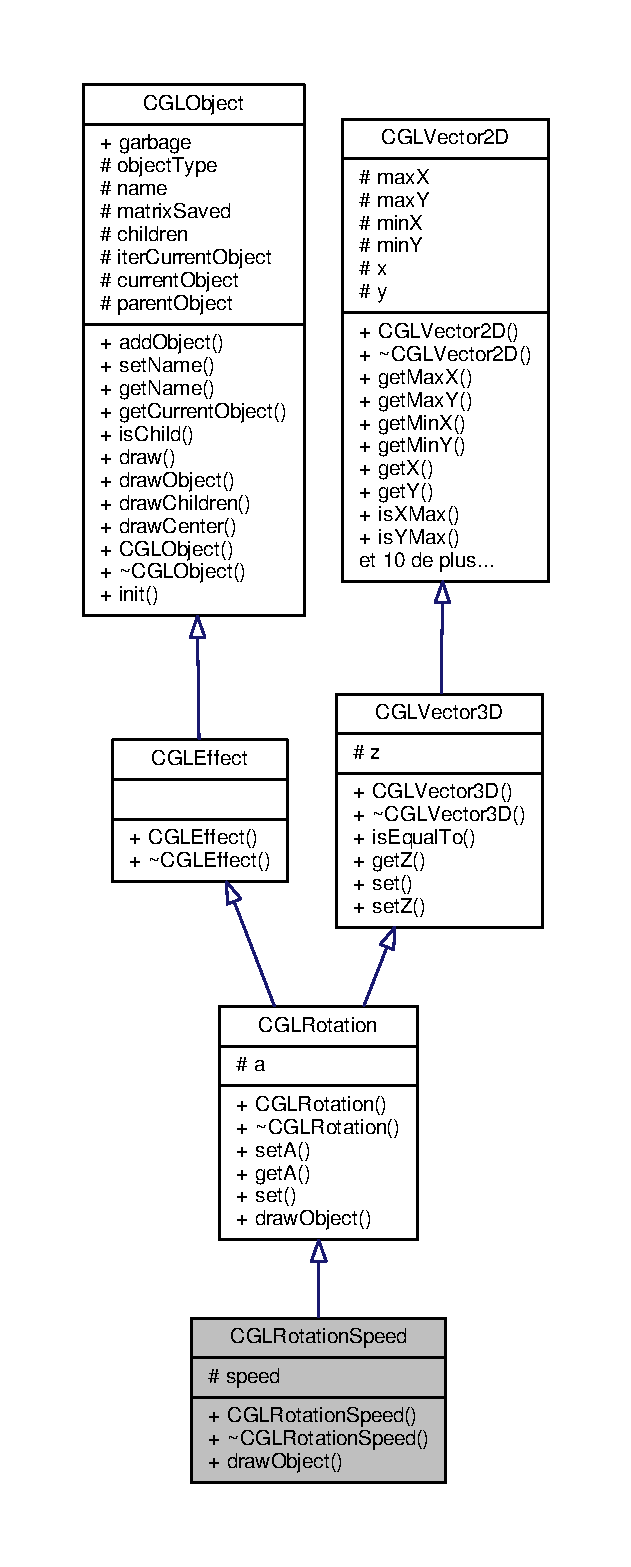
\includegraphics[height=550pt]{d0/dbb/class_c_g_l_rotation_speed__inherit__graph}
\end{center}
\end{figure}


Graphe de collaboration de C\-G\-L\-Rotation\-Speed\-:
\nopagebreak
\begin{figure}[H]
\begin{center}
\leavevmode
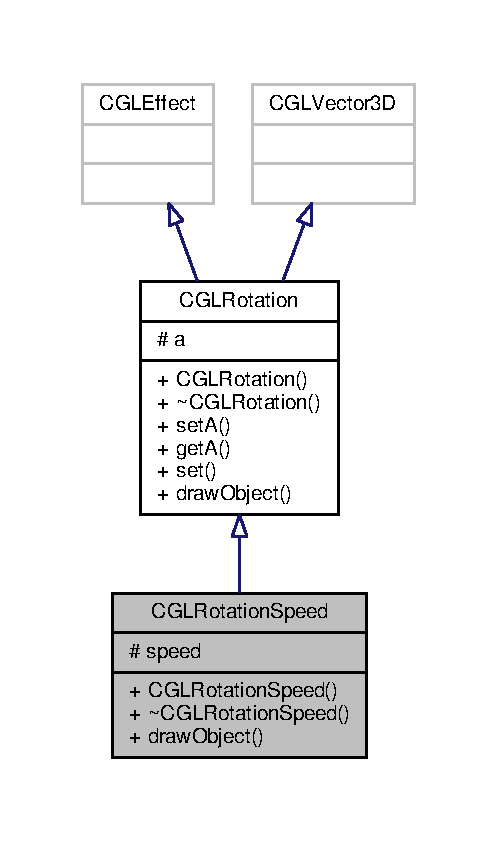
\includegraphics[height=550pt]{d1/dfb/class_c_g_l_rotation_speed__coll__graph}
\end{center}
\end{figure}
\subsection*{Fonctions membres publiques}
\begin{DoxyCompactItemize}
\item 
\hyperlink{class_c_g_l_rotation_speed_a6aed31b80ba1f7e050500469bf62e588}{C\-G\-L\-Rotation\-Speed} ()
\item 
virtual \hyperlink{class_c_g_l_rotation_speed_a7648604709da051825044630da6db987}{$\sim$\-C\-G\-L\-Rotation\-Speed} ()
\item 
void \hyperlink{class_c_g_l_rotation_speed_a6549d856fc0ad620fd1507744104797f}{draw\-Object} (Uint32 ellapsed\-Time)
\end{DoxyCompactItemize}
\subsection*{Attributs protégés}
\begin{DoxyCompactItemize}
\item 
double \hyperlink{class_c_g_l_rotation_speed_a5e9f478c8a0d828dac0ddee6777b45c4}{speed}
\end{DoxyCompactItemize}
\subsection*{Membres hérités additionnels}


\subsection{Description détaillée}


Définition à la ligne 17 du fichier C\-G\-L\-Rotation\-Speed.\-h.



\subsection{Documentation des constructeurs et destructeur}
\hypertarget{class_c_g_l_rotation_speed_a6aed31b80ba1f7e050500469bf62e588}{\index{C\-G\-L\-Rotation\-Speed@{C\-G\-L\-Rotation\-Speed}!C\-G\-L\-Rotation\-Speed@{C\-G\-L\-Rotation\-Speed}}
\index{C\-G\-L\-Rotation\-Speed@{C\-G\-L\-Rotation\-Speed}!CGLRotationSpeed@{C\-G\-L\-Rotation\-Speed}}
\subsubsection[{C\-G\-L\-Rotation\-Speed}]{\setlength{\rightskip}{0pt plus 5cm}C\-G\-L\-Rotation\-Speed\-::\-C\-G\-L\-Rotation\-Speed (
\begin{DoxyParamCaption}
{}
\end{DoxyParamCaption}
)}}\label{class_c_g_l_rotation_speed_a6aed31b80ba1f7e050500469bf62e588}


Définition à la ligne 10 du fichier C\-G\-L\-Rotation\-Speed.\-cpp.

\hypertarget{class_c_g_l_rotation_speed_a7648604709da051825044630da6db987}{\index{C\-G\-L\-Rotation\-Speed@{C\-G\-L\-Rotation\-Speed}!$\sim$\-C\-G\-L\-Rotation\-Speed@{$\sim$\-C\-G\-L\-Rotation\-Speed}}
\index{$\sim$\-C\-G\-L\-Rotation\-Speed@{$\sim$\-C\-G\-L\-Rotation\-Speed}!CGLRotationSpeed@{C\-G\-L\-Rotation\-Speed}}
\subsubsection[{$\sim$\-C\-G\-L\-Rotation\-Speed}]{\setlength{\rightskip}{0pt plus 5cm}C\-G\-L\-Rotation\-Speed\-::$\sim$\-C\-G\-L\-Rotation\-Speed (
\begin{DoxyParamCaption}
{}
\end{DoxyParamCaption}
)\hspace{0.3cm}{\ttfamily [virtual]}}}\label{class_c_g_l_rotation_speed_a7648604709da051825044630da6db987}


Définition à la ligne 14 du fichier C\-G\-L\-Rotation\-Speed.\-cpp.



\subsection{Documentation des fonctions membres}
\hypertarget{class_c_g_l_rotation_speed_a6549d856fc0ad620fd1507744104797f}{\index{C\-G\-L\-Rotation\-Speed@{C\-G\-L\-Rotation\-Speed}!draw\-Object@{draw\-Object}}
\index{draw\-Object@{draw\-Object}!CGLRotationSpeed@{C\-G\-L\-Rotation\-Speed}}
\subsubsection[{draw\-Object}]{\setlength{\rightskip}{0pt plus 5cm}void C\-G\-L\-Rotation\-Speed\-::draw\-Object (
\begin{DoxyParamCaption}
\item[{Uint32}]{ellapsed\-Time}
\end{DoxyParamCaption}
)\hspace{0.3cm}{\ttfamily [virtual]}}}\label{class_c_g_l_rotation_speed_a6549d856fc0ad620fd1507744104797f}


Réimplémentée à partir de \hyperlink{class_c_g_l_rotation_a94be2c089fbe52d0f8cb33ee98f8de74}{C\-G\-L\-Rotation}.



Définition à la ligne 18 du fichier C\-G\-L\-Rotation\-Speed.\-cpp.



Voici le graphe d'appel pour cette fonction \-:
\nopagebreak
\begin{figure}[H]
\begin{center}
\leavevmode
\includegraphics[width=350pt]{d4/d9e/class_c_g_l_rotation_speed_a6549d856fc0ad620fd1507744104797f_cgraph}
\end{center}
\end{figure}




\subsection{Documentation des données membres}
\hypertarget{class_c_g_l_rotation_speed_a5e9f478c8a0d828dac0ddee6777b45c4}{\index{C\-G\-L\-Rotation\-Speed@{C\-G\-L\-Rotation\-Speed}!speed@{speed}}
\index{speed@{speed}!CGLRotationSpeed@{C\-G\-L\-Rotation\-Speed}}
\subsubsection[{speed}]{\setlength{\rightskip}{0pt plus 5cm}double C\-G\-L\-Rotation\-Speed\-::speed\hspace{0.3cm}{\ttfamily [protected]}}}\label{class_c_g_l_rotation_speed_a5e9f478c8a0d828dac0ddee6777b45c4}


Définition à la ligne 20 du fichier C\-G\-L\-Rotation\-Speed.\-h.



La documentation de cette classe a été générée à partir des fichiers suivants \-:\begin{DoxyCompactItemize}
\item 
/home/dagal/git/\-Damier\-G\-L/\-Damier\-G\-L/src/\-C\-G\-L/\hyperlink{_c_g_l_rotation_speed_8h}{C\-G\-L\-Rotation\-Speed.\-h}\item 
/home/dagal/git/\-Damier\-G\-L/\-Damier\-G\-L/src/\-C\-G\-L/\hyperlink{_c_g_l_rotation_speed_8cpp}{C\-G\-L\-Rotation\-Speed.\-cpp}\end{DoxyCompactItemize}

\hypertarget{class_c_g_l_scale}{\section{Référence de la classe C\-G\-L\-Scale}
\label{class_c_g_l_scale}\index{C\-G\-L\-Scale@{C\-G\-L\-Scale}}
}


{\ttfamily \#include $<$C\-G\-L\-Scale.\-h$>$}



Graphe d'héritage de C\-G\-L\-Scale\-:
\nopagebreak
\begin{figure}[H]
\begin{center}
\leavevmode
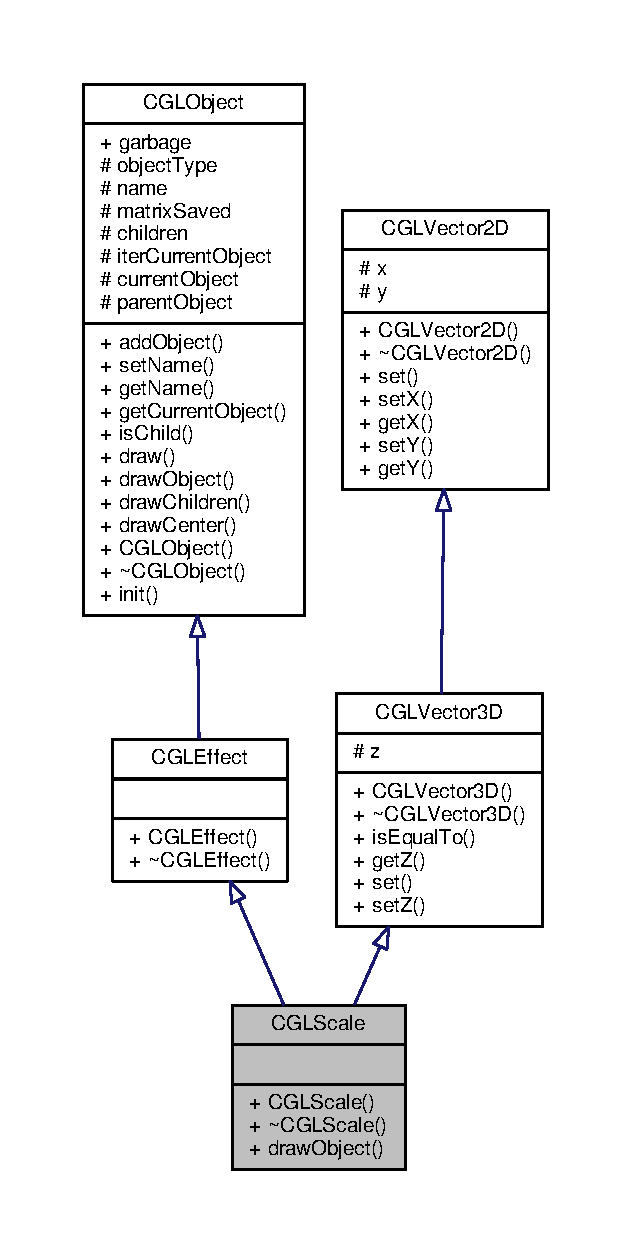
\includegraphics[height=550pt]{d9/d69/class_c_g_l_scale__inherit__graph}
\end{center}
\end{figure}


Graphe de collaboration de C\-G\-L\-Scale\-:
\nopagebreak
\begin{figure}[H]
\begin{center}
\leavevmode
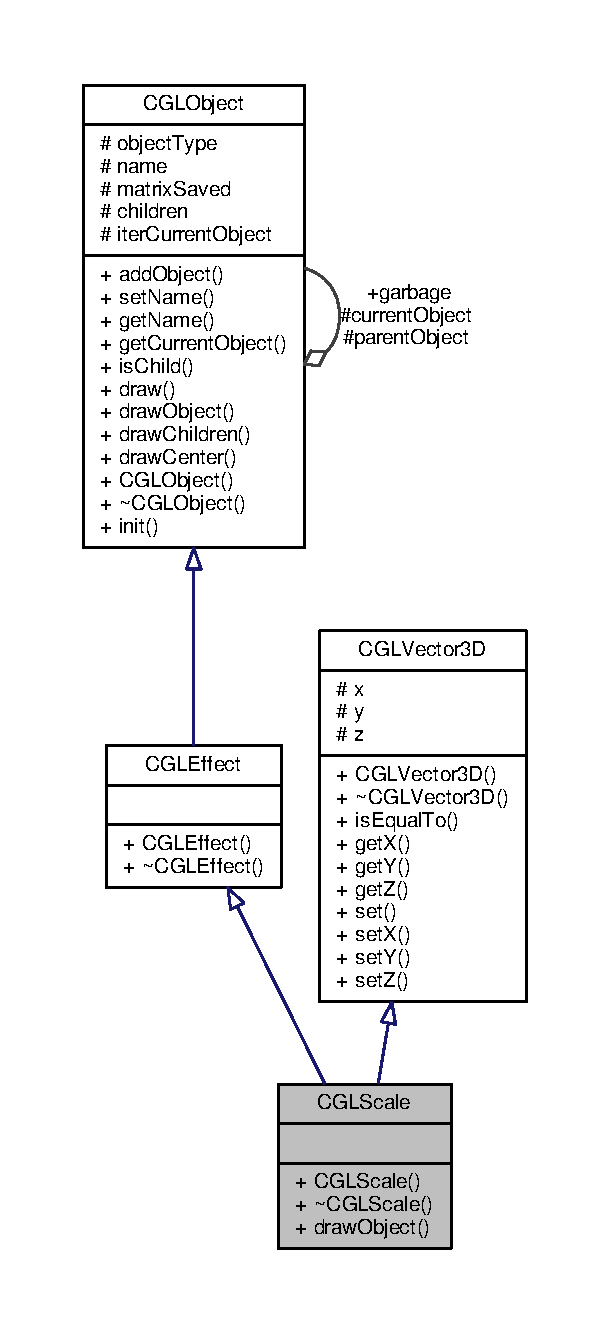
\includegraphics[width=350pt]{dd/d3a/class_c_g_l_scale__coll__graph}
\end{center}
\end{figure}
\subsection*{Fonctions membres publiques}
\begin{DoxyCompactItemize}
\item 
\hyperlink{class_c_g_l_scale_a48ed3886215e1ee3ae43fedae36cf426}{C\-G\-L\-Scale} ()
\item 
virtual \hyperlink{class_c_g_l_scale_a8a084fe6407bc5226723dd6300089cce}{$\sim$\-C\-G\-L\-Scale} ()
\item 
void \hyperlink{class_c_g_l_scale_a27939db2fb5f900800f391bb06a387a4}{draw\-Object} (Uint32 ellapsed\-Time)
\end{DoxyCompactItemize}
\subsection*{Membres hérités additionnels}


\subsection{Description détaillée}


Définition à la ligne 17 du fichier C\-G\-L\-Scale.\-h.



\subsection{Documentation des constructeurs et destructeur}
\hypertarget{class_c_g_l_scale_a48ed3886215e1ee3ae43fedae36cf426}{\index{C\-G\-L\-Scale@{C\-G\-L\-Scale}!C\-G\-L\-Scale@{C\-G\-L\-Scale}}
\index{C\-G\-L\-Scale@{C\-G\-L\-Scale}!CGLScale@{C\-G\-L\-Scale}}
\subsubsection[{C\-G\-L\-Scale}]{\setlength{\rightskip}{0pt plus 5cm}C\-G\-L\-Scale\-::\-C\-G\-L\-Scale (
\begin{DoxyParamCaption}
{}
\end{DoxyParamCaption}
)}}\label{class_c_g_l_scale_a48ed3886215e1ee3ae43fedae36cf426}


Définition à la ligne 10 du fichier C\-G\-L\-Scale.\-cpp.

\hypertarget{class_c_g_l_scale_a8a084fe6407bc5226723dd6300089cce}{\index{C\-G\-L\-Scale@{C\-G\-L\-Scale}!$\sim$\-C\-G\-L\-Scale@{$\sim$\-C\-G\-L\-Scale}}
\index{$\sim$\-C\-G\-L\-Scale@{$\sim$\-C\-G\-L\-Scale}!CGLScale@{C\-G\-L\-Scale}}
\subsubsection[{$\sim$\-C\-G\-L\-Scale}]{\setlength{\rightskip}{0pt plus 5cm}C\-G\-L\-Scale\-::$\sim$\-C\-G\-L\-Scale (
\begin{DoxyParamCaption}
{}
\end{DoxyParamCaption}
)\hspace{0.3cm}{\ttfamily [virtual]}}}\label{class_c_g_l_scale_a8a084fe6407bc5226723dd6300089cce}


Définition à la ligne 15 du fichier C\-G\-L\-Scale.\-cpp.



\subsection{Documentation des fonctions membres}
\hypertarget{class_c_g_l_scale_a27939db2fb5f900800f391bb06a387a4}{\index{C\-G\-L\-Scale@{C\-G\-L\-Scale}!draw\-Object@{draw\-Object}}
\index{draw\-Object@{draw\-Object}!CGLScale@{C\-G\-L\-Scale}}
\subsubsection[{draw\-Object}]{\setlength{\rightskip}{0pt plus 5cm}void C\-G\-L\-Scale\-::draw\-Object (
\begin{DoxyParamCaption}
\item[{Uint32}]{ellapsed\-Time}
\end{DoxyParamCaption}
)\hspace{0.3cm}{\ttfamily [virtual]}}}\label{class_c_g_l_scale_a27939db2fb5f900800f391bb06a387a4}


Réimplémentée à partir de \hyperlink{class_c_g_l_object_a2781ec98c37bd209f2382c5130a365b9}{C\-G\-L\-Object}.



Définition à la ligne 19 du fichier C\-G\-L\-Scale.\-cpp.



La documentation de cette classe a été générée à partir des fichiers suivants \-:\begin{DoxyCompactItemize}
\item 
/home/dagal/git/\-Damier\-G\-L/\-Damier\-G\-L/src/\-C\-G\-L/\hyperlink{_c_g_l_scale_8h}{C\-G\-L\-Scale.\-h}\item 
/home/dagal/git/\-Damier\-G\-L/\-Damier\-G\-L/src/\-C\-G\-L/\hyperlink{_c_g_l_scale_8cpp}{C\-G\-L\-Scale.\-cpp}\end{DoxyCompactItemize}

\hypertarget{class_c_g_l_triangle}{\section{Référence de la classe C\-G\-L\-Triangle}
\label{class_c_g_l_triangle}\index{C\-G\-L\-Triangle@{C\-G\-L\-Triangle}}
}


{\ttfamily \#include $<$C\-G\-L\-Triangle.\-h$>$}



Graphe d'héritage de C\-G\-L\-Triangle\-:\nopagebreak
\begin{figure}[H]
\begin{center}
\leavevmode
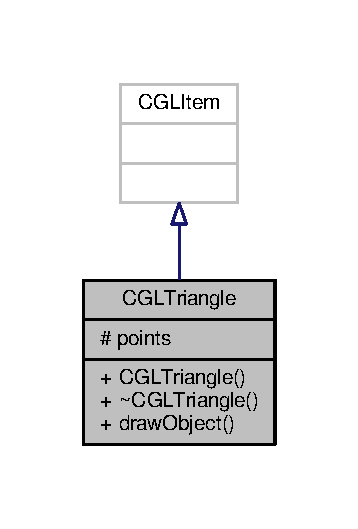
\includegraphics[height=550pt]{dd/d84/class_c_g_l_triangle__inherit__graph}
\end{center}
\end{figure}


Graphe de collaboration de C\-G\-L\-Triangle\-:
\nopagebreak
\begin{figure}[H]
\begin{center}
\leavevmode
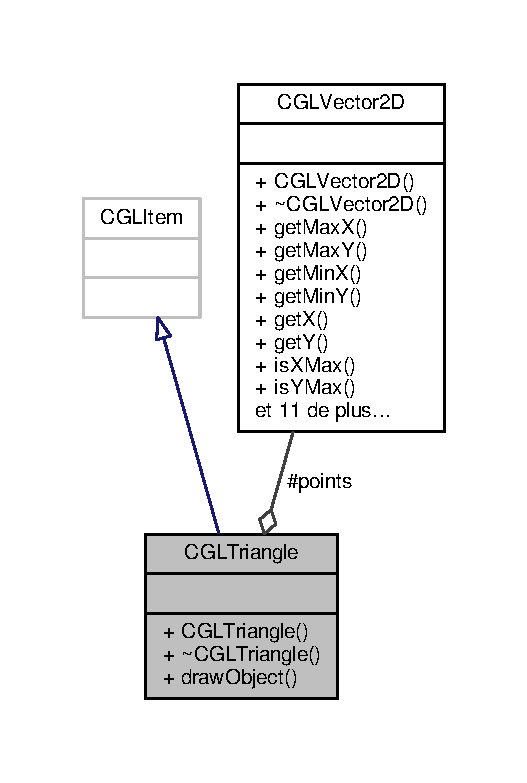
\includegraphics[height=550pt]{d5/d01/class_c_g_l_triangle__coll__graph}
\end{center}
\end{figure}
\subsection*{Fonctions membres publiques}
\begin{DoxyCompactItemize}
\item 
\hyperlink{class_c_g_l_triangle_a4b704efe008da14c3fc290ca86dc4b8c}{C\-G\-L\-Triangle} ()
\item 
virtual \hyperlink{class_c_g_l_triangle_a5dae52a9a0c14104d2ee82ad4cb859e9}{$\sim$\-C\-G\-L\-Triangle} ()
\item 
void \hyperlink{class_c_g_l_triangle_aab44f7f6fca4ad4cca693205aeb92fe3}{draw\-Object} (Uint32 ellapsed\-Time)
\end{DoxyCompactItemize}
\subsection*{Attributs protégés}
\begin{DoxyCompactItemize}
\item 
\hyperlink{class_c_g_l_vector2_d}{C\-G\-L\-Vector2\-D} \hyperlink{class_c_g_l_triangle_ad9fa3aa96d255554fe524c3e1aa68cee}{points} \mbox{[}3\mbox{]}
\end{DoxyCompactItemize}
\subsection*{Membres hérités additionnels}


\subsection{Description détaillée}


Définition à la ligne 18 du fichier C\-G\-L\-Triangle.\-h.



\subsection{Documentation des constructeurs et destructeur}
\hypertarget{class_c_g_l_triangle_a4b704efe008da14c3fc290ca86dc4b8c}{\index{C\-G\-L\-Triangle@{C\-G\-L\-Triangle}!C\-G\-L\-Triangle@{C\-G\-L\-Triangle}}
\index{C\-G\-L\-Triangle@{C\-G\-L\-Triangle}!CGLTriangle@{C\-G\-L\-Triangle}}
\subsubsection[{C\-G\-L\-Triangle}]{\setlength{\rightskip}{0pt plus 5cm}C\-G\-L\-Triangle\-::\-C\-G\-L\-Triangle (
\begin{DoxyParamCaption}
{}
\end{DoxyParamCaption}
)}}\label{class_c_g_l_triangle_a4b704efe008da14c3fc290ca86dc4b8c}


Définition à la ligne 10 du fichier C\-G\-L\-Triangle.\-cpp.



Voici le graphe d'appel pour cette fonction \-:\nopagebreak
\begin{figure}[H]
\begin{center}
\leavevmode
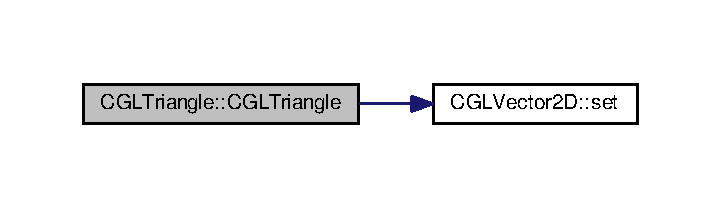
\includegraphics[width=350pt]{d1/d68/class_c_g_l_triangle_a4b704efe008da14c3fc290ca86dc4b8c_cgraph}
\end{center}
\end{figure}


\hypertarget{class_c_g_l_triangle_a5dae52a9a0c14104d2ee82ad4cb859e9}{\index{C\-G\-L\-Triangle@{C\-G\-L\-Triangle}!$\sim$\-C\-G\-L\-Triangle@{$\sim$\-C\-G\-L\-Triangle}}
\index{$\sim$\-C\-G\-L\-Triangle@{$\sim$\-C\-G\-L\-Triangle}!CGLTriangle@{C\-G\-L\-Triangle}}
\subsubsection[{$\sim$\-C\-G\-L\-Triangle}]{\setlength{\rightskip}{0pt plus 5cm}C\-G\-L\-Triangle\-::$\sim$\-C\-G\-L\-Triangle (
\begin{DoxyParamCaption}
{}
\end{DoxyParamCaption}
)\hspace{0.3cm}{\ttfamily [virtual]}}}\label{class_c_g_l_triangle_a5dae52a9a0c14104d2ee82ad4cb859e9}


Définition à la ligne 17 du fichier C\-G\-L\-Triangle.\-cpp.



\subsection{Documentation des fonctions membres}
\hypertarget{class_c_g_l_triangle_aab44f7f6fca4ad4cca693205aeb92fe3}{\index{C\-G\-L\-Triangle@{C\-G\-L\-Triangle}!draw\-Object@{draw\-Object}}
\index{draw\-Object@{draw\-Object}!CGLTriangle@{C\-G\-L\-Triangle}}
\subsubsection[{draw\-Object}]{\setlength{\rightskip}{0pt plus 5cm}void C\-G\-L\-Triangle\-::draw\-Object (
\begin{DoxyParamCaption}
\item[{Uint32}]{ellapsed\-Time}
\end{DoxyParamCaption}
)\hspace{0.3cm}{\ttfamily [virtual]}}}\label{class_c_g_l_triangle_aab44f7f6fca4ad4cca693205aeb92fe3}


Réimplémentée à partir de \hyperlink{class_c_g_l_object_a2781ec98c37bd209f2382c5130a365b9}{C\-G\-L\-Object}.



Définition à la ligne 21 du fichier C\-G\-L\-Triangle.\-cpp.



\subsection{Documentation des données membres}
\hypertarget{class_c_g_l_triangle_ad9fa3aa96d255554fe524c3e1aa68cee}{\index{C\-G\-L\-Triangle@{C\-G\-L\-Triangle}!points@{points}}
\index{points@{points}!CGLTriangle@{C\-G\-L\-Triangle}}
\subsubsection[{points}]{\setlength{\rightskip}{0pt plus 5cm}{\bf C\-G\-L\-Vector2\-D} C\-G\-L\-Triangle\-::points\mbox{[}3\mbox{]}\hspace{0.3cm}{\ttfamily [protected]}}}\label{class_c_g_l_triangle_ad9fa3aa96d255554fe524c3e1aa68cee}


Définition à la ligne 21 du fichier C\-G\-L\-Triangle.\-h.



La documentation de cette classe a été générée à partir des fichiers suivants \-:\begin{DoxyCompactItemize}
\item 
/home/dagal/git/\-Damier\-G\-L/\-Damier\-G\-L/src/\-C\-G\-L/\hyperlink{_c_g_l_triangle_8h}{C\-G\-L\-Triangle.\-h}\item 
/home/dagal/git/\-Damier\-G\-L/\-Damier\-G\-L/src/\-C\-G\-L/\hyperlink{_c_g_l_triangle_8cpp}{C\-G\-L\-Triangle.\-cpp}\end{DoxyCompactItemize}

\hypertarget{class_c_g_l_vector2_d}{\section{Référence de la classe C\-G\-L\-Vector2\-D}
\label{class_c_g_l_vector2_d}\index{C\-G\-L\-Vector2\-D@{C\-G\-L\-Vector2\-D}}
}


{\ttfamily \#include $<$C\-G\-L\-Vector2\-D.\-h$>$}



Graphe d'héritage de C\-G\-L\-Vector2\-D\-:
\nopagebreak
\begin{figure}[H]
\begin{center}
\leavevmode
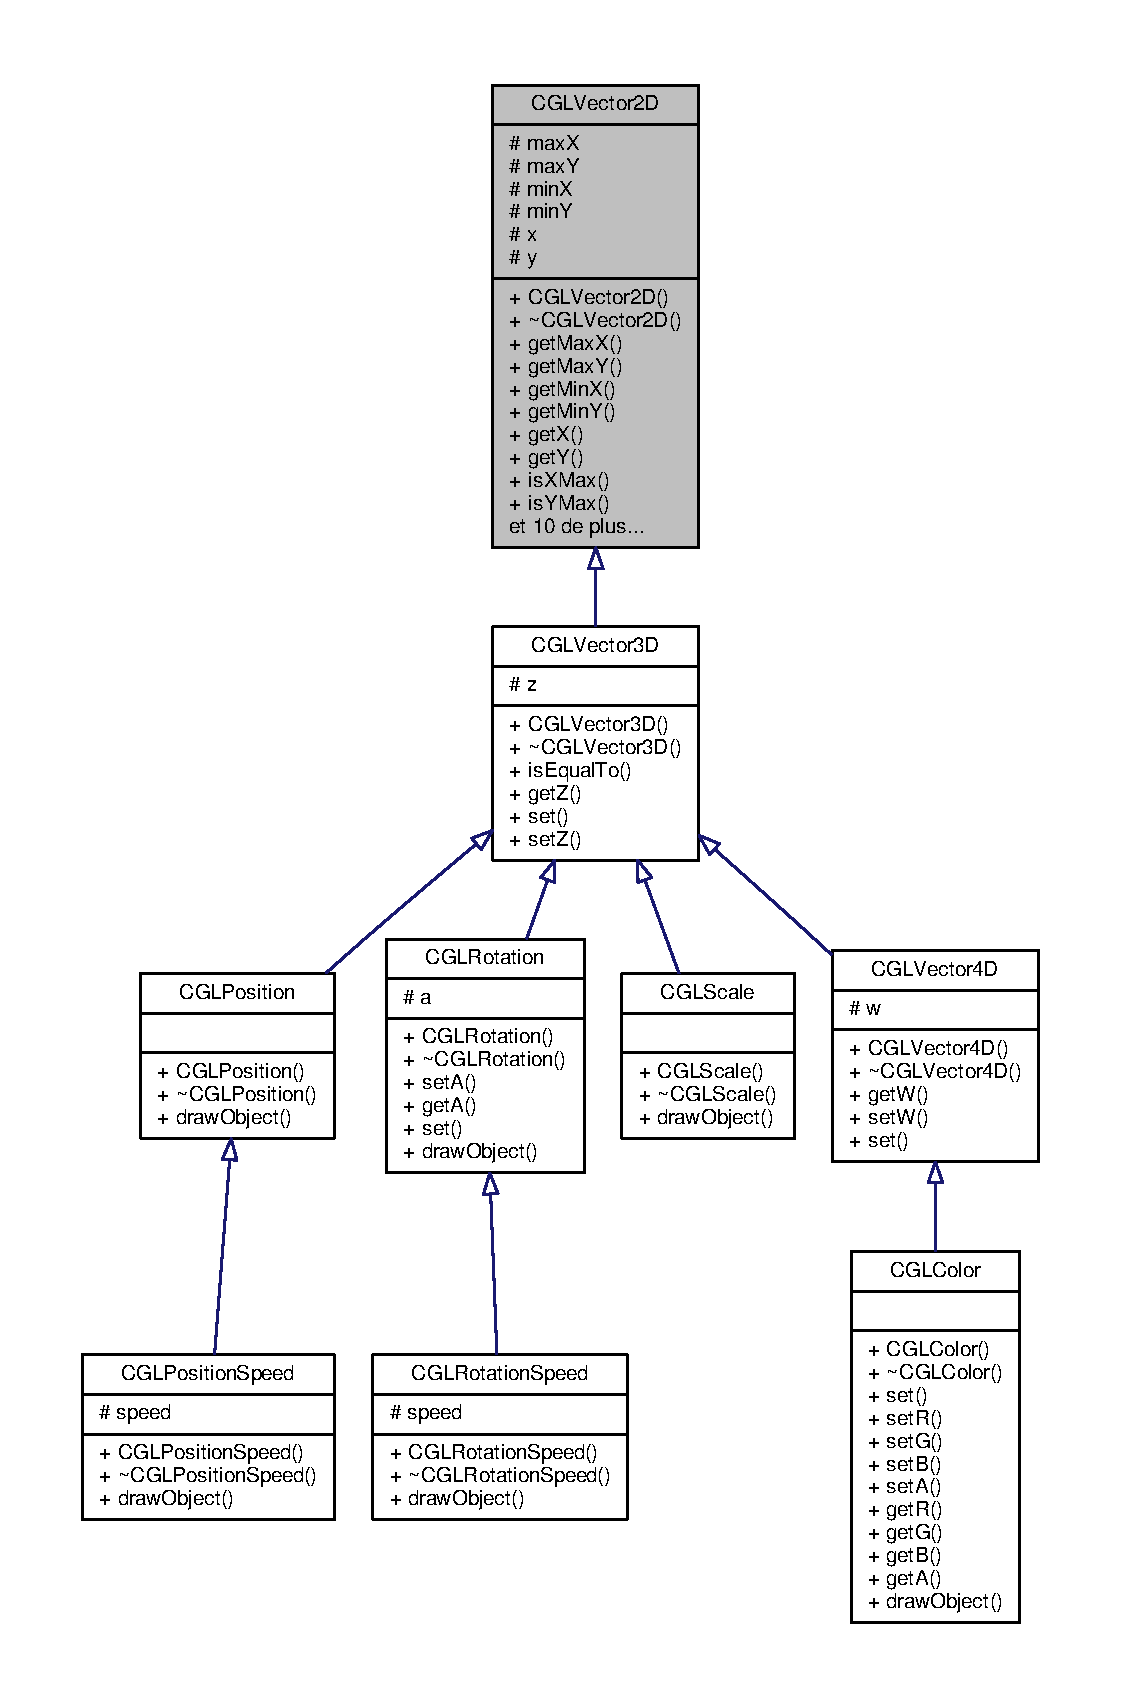
\includegraphics[width=350pt]{d2/def/class_c_g_l_vector2_d__inherit__graph}
\end{center}
\end{figure}


Graphe de collaboration de C\-G\-L\-Vector2\-D\-:
\nopagebreak
\begin{figure}[H]
\begin{center}
\leavevmode
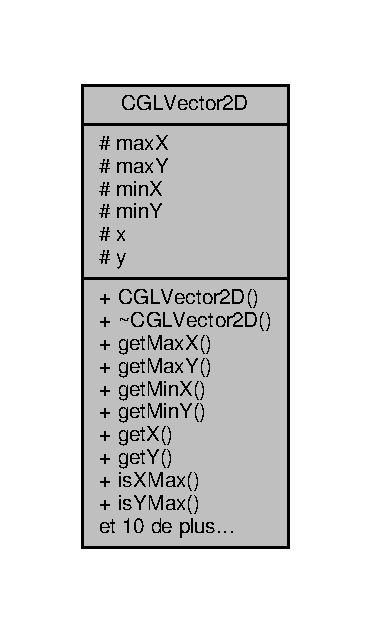
\includegraphics[width=178pt]{db/d79/class_c_g_l_vector2_d__coll__graph}
\end{center}
\end{figure}
\subsection*{Fonctions membres publiques}
\begin{DoxyCompactItemize}
\item 
\hyperlink{class_c_g_l_vector2_d_a777d33ddc05a95c0c4a56672d50a3138}{C\-G\-L\-Vector2\-D} ()
\item 
virtual \hyperlink{class_c_g_l_vector2_d_a93cf12a834078803bee4f19d42e09a02}{$\sim$\-C\-G\-L\-Vector2\-D} ()
\item 
void \hyperlink{class_c_g_l_vector2_d_a37b79a5ca7b3445df956e177f7c436fc}{set} (double const \&valx, double const \&valy)
\item 
void \hyperlink{class_c_g_l_vector2_d_a22db1a511fae81b0d7a6766b6490dd8c}{set\-X} (double const \&val)
\item 
double const \& \hyperlink{class_c_g_l_vector2_d_a5f25e872259c579251336dfe0faf8701}{get\-X} () const 
\item 
void \hyperlink{class_c_g_l_vector2_d_a4c89a21e28a86848c6b023ad60baef4c}{set\-Y} (double const \&val)
\item 
double const \& \hyperlink{class_c_g_l_vector2_d_ad279638b74a0caac60632b169136688c}{get\-Y} () const 
\end{DoxyCompactItemize}
\subsection*{Attributs protégés}
\begin{DoxyCompactItemize}
\item 
double \hyperlink{class_c_g_l_vector2_d_adca68a6660d264b4fcb312c881c57861}{x}
\item 
double \hyperlink{class_c_g_l_vector2_d_a36a88cf9827f308a125e51164c73e21f}{y}
\end{DoxyCompactItemize}


\subsection{Description détaillée}


Définition à la ligne 15 du fichier C\-G\-L\-Vector2\-D.\-h.



\subsection{Documentation des constructeurs et destructeur}
\hypertarget{class_c_g_l_vector2_d_a777d33ddc05a95c0c4a56672d50a3138}{\index{C\-G\-L\-Vector2\-D@{C\-G\-L\-Vector2\-D}!C\-G\-L\-Vector2\-D@{C\-G\-L\-Vector2\-D}}
\index{C\-G\-L\-Vector2\-D@{C\-G\-L\-Vector2\-D}!CGLVector2D@{C\-G\-L\-Vector2\-D}}
\subsubsection[{C\-G\-L\-Vector2\-D}]{\setlength{\rightskip}{0pt plus 5cm}C\-G\-L\-Vector2\-D\-::\-C\-G\-L\-Vector2\-D (
\begin{DoxyParamCaption}
{}
\end{DoxyParamCaption}
)}}\label{class_c_g_l_vector2_d_a777d33ddc05a95c0c4a56672d50a3138}


Définition à la ligne 10 du fichier C\-G\-L\-Vector2\-D.\-cpp.

\hypertarget{class_c_g_l_vector2_d_a93cf12a834078803bee4f19d42e09a02}{\index{C\-G\-L\-Vector2\-D@{C\-G\-L\-Vector2\-D}!$\sim$\-C\-G\-L\-Vector2\-D@{$\sim$\-C\-G\-L\-Vector2\-D}}
\index{$\sim$\-C\-G\-L\-Vector2\-D@{$\sim$\-C\-G\-L\-Vector2\-D}!CGLVector2D@{C\-G\-L\-Vector2\-D}}
\subsubsection[{$\sim$\-C\-G\-L\-Vector2\-D}]{\setlength{\rightskip}{0pt plus 5cm}C\-G\-L\-Vector2\-D\-::$\sim$\-C\-G\-L\-Vector2\-D (
\begin{DoxyParamCaption}
{}
\end{DoxyParamCaption}
)\hspace{0.3cm}{\ttfamily [virtual]}}}\label{class_c_g_l_vector2_d_a93cf12a834078803bee4f19d42e09a02}


Définition à la ligne 16 du fichier C\-G\-L\-Vector2\-D.\-cpp.



\subsection{Documentation des fonctions membres}
\hypertarget{class_c_g_l_vector2_d_a5f25e872259c579251336dfe0faf8701}{\index{C\-G\-L\-Vector2\-D@{C\-G\-L\-Vector2\-D}!get\-X@{get\-X}}
\index{get\-X@{get\-X}!CGLVector2D@{C\-G\-L\-Vector2\-D}}
\subsubsection[{get\-X}]{\setlength{\rightskip}{0pt plus 5cm}double const \& C\-G\-L\-Vector2\-D\-::get\-X (
\begin{DoxyParamCaption}
{}
\end{DoxyParamCaption}
) const}}\label{class_c_g_l_vector2_d_a5f25e872259c579251336dfe0faf8701}


Définition à la ligne 36 du fichier C\-G\-L\-Vector2\-D.\-cpp.



Voici le graphe des appelants de cette fonction \-:
\nopagebreak
\begin{figure}[H]
\begin{center}
\leavevmode
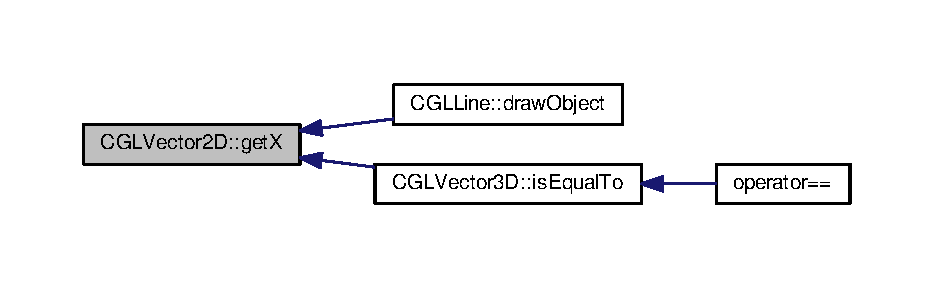
\includegraphics[width=350pt]{d8/d97/class_c_g_l_vector2_d_a5f25e872259c579251336dfe0faf8701_icgraph}
\end{center}
\end{figure}


\hypertarget{class_c_g_l_vector2_d_ad279638b74a0caac60632b169136688c}{\index{C\-G\-L\-Vector2\-D@{C\-G\-L\-Vector2\-D}!get\-Y@{get\-Y}}
\index{get\-Y@{get\-Y}!CGLVector2D@{C\-G\-L\-Vector2\-D}}
\subsubsection[{get\-Y}]{\setlength{\rightskip}{0pt plus 5cm}double const \& C\-G\-L\-Vector2\-D\-::get\-Y (
\begin{DoxyParamCaption}
{}
\end{DoxyParamCaption}
) const}}\label{class_c_g_l_vector2_d_ad279638b74a0caac60632b169136688c}


Définition à la ligne 41 du fichier C\-G\-L\-Vector2\-D.\-cpp.



Voici le graphe des appelants de cette fonction \-:
\nopagebreak
\begin{figure}[H]
\begin{center}
\leavevmode
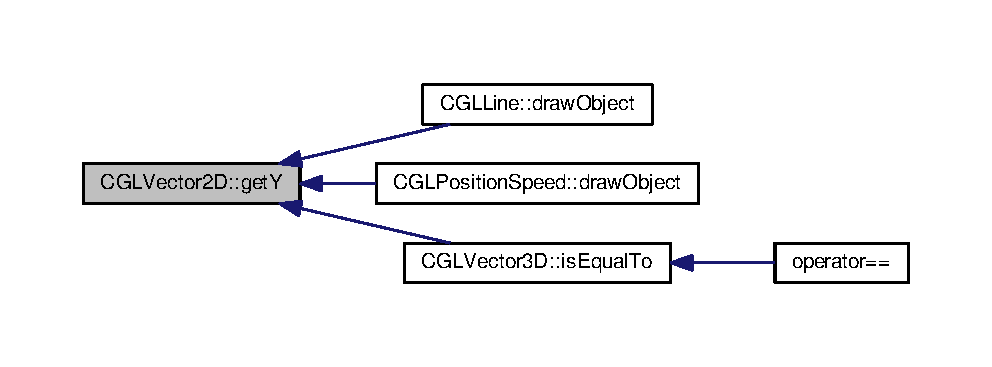
\includegraphics[width=350pt]{d8/d97/class_c_g_l_vector2_d_ad279638b74a0caac60632b169136688c_icgraph}
\end{center}
\end{figure}


\hypertarget{class_c_g_l_vector2_d_a37b79a5ca7b3445df956e177f7c436fc}{\index{C\-G\-L\-Vector2\-D@{C\-G\-L\-Vector2\-D}!set@{set}}
\index{set@{set}!CGLVector2D@{C\-G\-L\-Vector2\-D}}
\subsubsection[{set}]{\setlength{\rightskip}{0pt plus 5cm}void C\-G\-L\-Vector2\-D\-::set (
\begin{DoxyParamCaption}
\item[{double const \&}]{valx, }
\item[{double const \&}]{valy}
\end{DoxyParamCaption}
)}}\label{class_c_g_l_vector2_d_a37b79a5ca7b3445df956e177f7c436fc}


Définition à la ligne 20 du fichier C\-G\-L\-Vector2\-D.\-cpp.



Voici le graphe des appelants de cette fonction \-:
\nopagebreak
\begin{figure}[H]
\begin{center}
\leavevmode
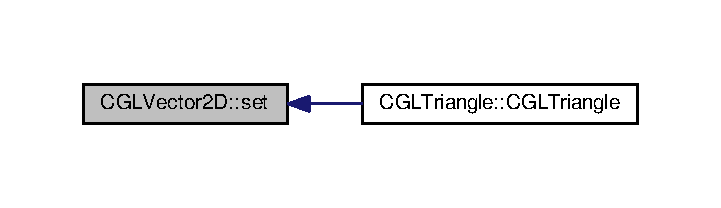
\includegraphics[width=346pt]{d8/d97/class_c_g_l_vector2_d_a37b79a5ca7b3445df956e177f7c436fc_icgraph}
\end{center}
\end{figure}


\hypertarget{class_c_g_l_vector2_d_a22db1a511fae81b0d7a6766b6490dd8c}{\index{C\-G\-L\-Vector2\-D@{C\-G\-L\-Vector2\-D}!set\-X@{set\-X}}
\index{set\-X@{set\-X}!CGLVector2D@{C\-G\-L\-Vector2\-D}}
\subsubsection[{set\-X}]{\setlength{\rightskip}{0pt plus 5cm}void C\-G\-L\-Vector2\-D\-::set\-X (
\begin{DoxyParamCaption}
\item[{double const \&}]{val}
\end{DoxyParamCaption}
)}}\label{class_c_g_l_vector2_d_a22db1a511fae81b0d7a6766b6490dd8c}


Définition à la ligne 26 du fichier C\-G\-L\-Vector2\-D.\-cpp.

\hypertarget{class_c_g_l_vector2_d_a4c89a21e28a86848c6b023ad60baef4c}{\index{C\-G\-L\-Vector2\-D@{C\-G\-L\-Vector2\-D}!set\-Y@{set\-Y}}
\index{set\-Y@{set\-Y}!CGLVector2D@{C\-G\-L\-Vector2\-D}}
\subsubsection[{set\-Y}]{\setlength{\rightskip}{0pt plus 5cm}void C\-G\-L\-Vector2\-D\-::set\-Y (
\begin{DoxyParamCaption}
\item[{double const \&}]{val}
\end{DoxyParamCaption}
)}}\label{class_c_g_l_vector2_d_a4c89a21e28a86848c6b023ad60baef4c}


Définition à la ligne 31 du fichier C\-G\-L\-Vector2\-D.\-cpp.



\subsection{Documentation des données membres}
\hypertarget{class_c_g_l_vector2_d_adca68a6660d264b4fcb312c881c57861}{\index{C\-G\-L\-Vector2\-D@{C\-G\-L\-Vector2\-D}!x@{x}}
\index{x@{x}!CGLVector2D@{C\-G\-L\-Vector2\-D}}
\subsubsection[{x}]{\setlength{\rightskip}{0pt plus 5cm}double C\-G\-L\-Vector2\-D\-::x\hspace{0.3cm}{\ttfamily [protected]}}}\label{class_c_g_l_vector2_d_adca68a6660d264b4fcb312c881c57861}


Définition à la ligne 18 du fichier C\-G\-L\-Vector2\-D.\-h.

\hypertarget{class_c_g_l_vector2_d_a36a88cf9827f308a125e51164c73e21f}{\index{C\-G\-L\-Vector2\-D@{C\-G\-L\-Vector2\-D}!y@{y}}
\index{y@{y}!CGLVector2D@{C\-G\-L\-Vector2\-D}}
\subsubsection[{y}]{\setlength{\rightskip}{0pt plus 5cm}double C\-G\-L\-Vector2\-D\-::y\hspace{0.3cm}{\ttfamily [protected]}}}\label{class_c_g_l_vector2_d_a36a88cf9827f308a125e51164c73e21f}


Définition à la ligne 19 du fichier C\-G\-L\-Vector2\-D.\-h.



La documentation de cette classe a été générée à partir des fichiers suivants \-:\begin{DoxyCompactItemize}
\item 
/home/dagal/git/\-Damier\-G\-L/\-Damier\-G\-L/src/\-C\-G\-L/\hyperlink{_c_g_l_vector2_d_8h}{C\-G\-L\-Vector2\-D.\-h}\item 
/home/dagal/git/\-Damier\-G\-L/\-Damier\-G\-L/src/\-C\-G\-L/\hyperlink{_c_g_l_vector2_d_8cpp}{C\-G\-L\-Vector2\-D.\-cpp}\end{DoxyCompactItemize}

\input{d0/d65/class_d_g_l_1_1_circle}
\input{d4/d56/class_d_g_l_1_1_color}
\input{de/d94/class_d_g_l_1_1_effect}
\input{d6/d83/class_d_g_l_1_1_item}
\input{da/d7c/class_light}
\input{dd/d66/class_d_g_l_1_1_object}
\input{d6/db5/class_scene}
\input{d9/dee/class_d_g_l_1_1_special}
\input{dc/db6/class_d_g_l_1_1_vector3_d}
\input{d9/d48/class_d_g_l_1_1_vector4_d}
\input{d1/d91/class_d_g_l_1_1_window}
\input{d3/d21/class_world}
\chapter{Documentation des fichiers}
\input{df/d0f/_box_8cpp}
\input{d0/d5c/_box_8h}
\input{d1/d33/_camera_8cpp}
\input{d5/d91/_camera_8h}
\input{d7/d4e/_camera_list_8cpp}
\input{db/da6/_camera_list_8h}
\input{d4/d94/_circle_8cpp}
\input{db/d50/_circle_8h}
\input{d0/d22/_color_8cpp}
\input{d9/df8/_color_8h}
\input{d5/dc5/_dot_8cpp}
\input{d3/d94/_dot_8h}
\input{d3/d3d/_effect_8cpp}
\input{dd/d44/_effect_8h}
\input{db/d54/_item_8cpp}
\input{da/d43/_item_8h}
\input{d5/d56/_light_8cpp}
\input{d2/d46/_light_8h}
\input{d0/d8a/_line_8cpp}
\input{d0/dee/_line_8h}
\input{d8/ded/_object_8cpp}
\input{df/d30/_object_8h}
\input{dd/d25/_polygon_8cpp}
\input{da/d08/_polygon_8h}
\input{db/d6d/_position_8cpp}
\input{d4/d51/_position_8h}
\input{d6/d22/_quad_8cpp}
\input{db/dc0/_quad_8h}
\input{da/d15/_robot1_8cpp}
\input{d7/daf/_robot1_8h}
\input{de/d4e/_rotation_8cpp}
\input{d9/dd4/_rotation_8h}
\input{d1/d44/_rotation_speed_8cpp}
\input{df/dd1/_rotation_speed_8h}
\input{d6/dc7/_scale_8cpp}
\input{d4/d81/_scale_8h}
\input{d9/d44/_scene_8cpp}
\input{de/d56/_scene_8h}
\input{d3/d9d/_special_8cpp}
\input{dd/da2/_special_8h}
\input{dd/ddc/_triangle_8cpp}
\input{db/de5/_triangle_8h}
\input{d9/d65/_vector2_d_8cpp}
\input{d1/dae/_vector2_d_8h}
\input{d8/d72/_vector3_d_8cpp}
\input{d6/d90/_vector3_d_8h}
\input{d9/da3/_vector4_d_8cpp}
\input{da/d5a/_vector4_d_8h}
\input{d3/db8/_window_8cpp}
\input{de/d42/_window_8h}
\input{d0/dd5/_world_8cpp}
\input{d8/d86/_world_8h}
\hypertarget{_damier_g_l_8cpp}{\section{Référence du fichier /home/dagal/git/\-Damier\-G\-L/\-Damier\-G\-L/src/\-Damier\-G\-L.cpp}
\label{_damier_g_l_8cpp}\index{/home/dagal/git/\-Damier\-G\-L/\-Damier\-G\-L/src/\-Damier\-G\-L.\-cpp@{/home/dagal/git/\-Damier\-G\-L/\-Damier\-G\-L/src/\-Damier\-G\-L.\-cpp}}
}
{\ttfamily \#include \char`\"{}C\-G\-L/\-C\-G\-L\-Window.\-h\char`\"{}}\\*
{\ttfamily \#include \char`\"{}C\-G\-L/\-C\-G\-L\-Quad.\-h\char`\"{}}\\*
{\ttfamily \#include \char`\"{}C\-G\-L/\-C\-G\-L\-Robot1.\-h\char`\"{}}\\*
{\ttfamily \#include \char`\"{}C\-G\-L/\-C\-G\-L\-Color.\-h\char`\"{}}\\*
{\ttfamily \#include \char`\"{}C\-G\-L/\-C\-G\-L\-Scale.\-h\char`\"{}}\\*
{\ttfamily \#include \char`\"{}C\-G\-L/\-C\-G\-L\-Dot.\-h\char`\"{}}\\*
{\ttfamily \#include \char`\"{}C\-G\-L/\-C\-G\-L\-Line.\-h\char`\"{}}\\*
{\ttfamily \#include \char`\"{}C\-G\-L/\-C\-G\-L\-Triangle.\-h\char`\"{}}\\*
{\ttfamily \#include \char`\"{}C\-G\-L/\-C\-G\-L\-Polygon.\-h\char`\"{}}\\*
{\ttfamily \#include \char`\"{}C\-G\-L/\-C\-G\-L\-Circle.\-h\char`\"{}}\\*
{\ttfamily \#include \char`\"{}C\-G\-L/\-C\-G\-L\-Position.\-h\char`\"{}}\\*
{\ttfamily \#include \char`\"{}C\-G\-L/\-C\-G\-L\-Rotation\-Speed.\-h\char`\"{}}\\*
Graphe des dépendances par inclusion de Damier\-G\-L.\-cpp\-:
\nopagebreak
\begin{figure}[H]
\begin{center}
\leavevmode
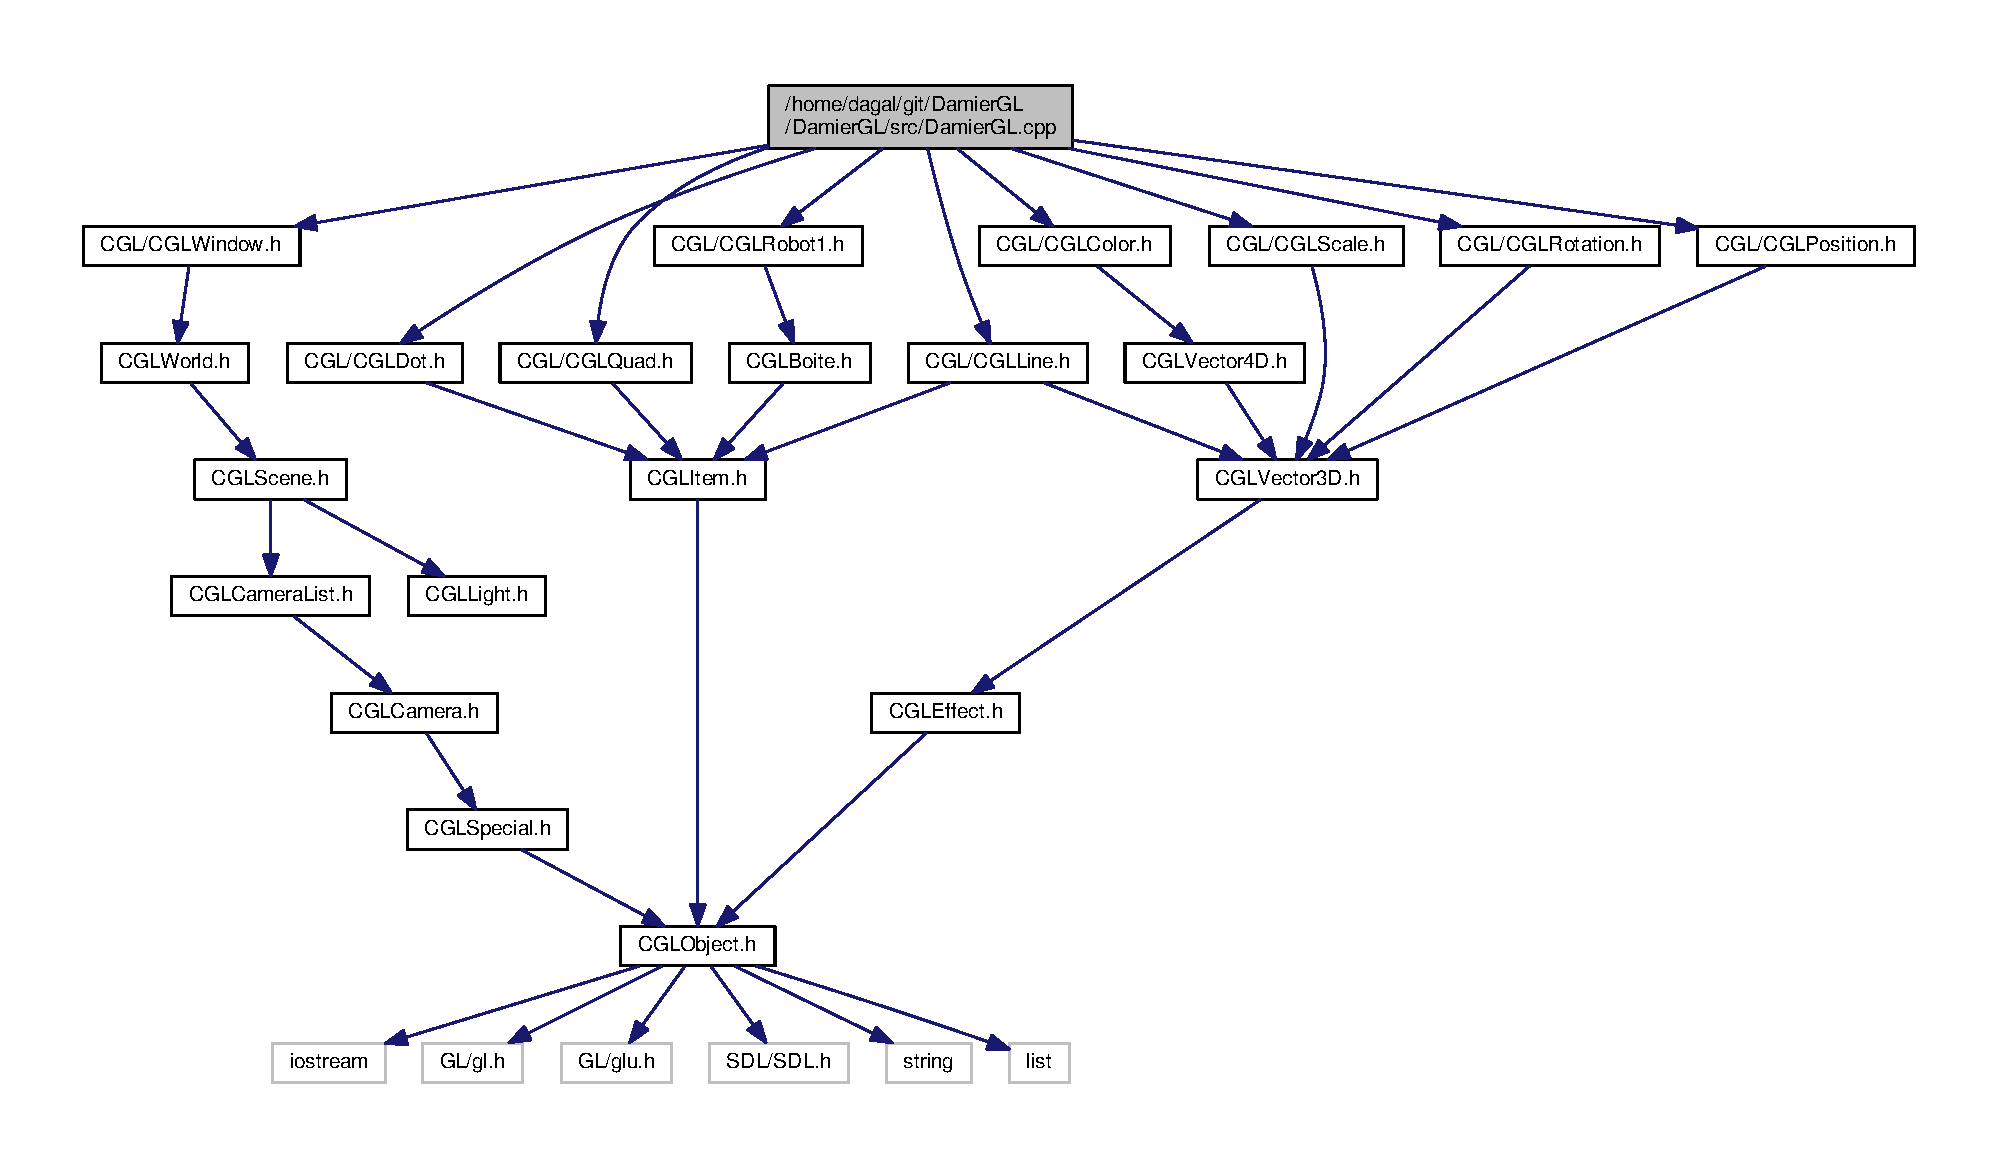
\includegraphics[width=350pt]{d9/dc9/_damier_g_l_8cpp__incl}
\end{center}
\end{figure}
\subsection*{Fonctions}
\begin{DoxyCompactItemize}
\item 
int \hyperlink{_damier_g_l_8cpp_a0ddf1224851353fc92bfbff6f499fa97}{main} (int argc, char $\ast$argv\mbox{[}$\,$\mbox{]})
\end{DoxyCompactItemize}


\subsection{Documentation des fonctions}
\hypertarget{_damier_g_l_8cpp_a0ddf1224851353fc92bfbff6f499fa97}{\index{Damier\-G\-L.\-cpp@{Damier\-G\-L.\-cpp}!main@{main}}
\index{main@{main}!DamierGL.cpp@{Damier\-G\-L.\-cpp}}
\subsubsection[{main}]{\setlength{\rightskip}{0pt plus 5cm}int main (
\begin{DoxyParamCaption}
\item[{int}]{argc, }
\item[{char $\ast$}]{argv\mbox{[}$\,$\mbox{]}}
\end{DoxyParamCaption}
)}}\label{_damier_g_l_8cpp_a0ddf1224851353fc92bfbff6f499fa97}


Définition à la ligne 22 du fichier Damier\-G\-L.\-cpp.



Voici le graphe d'appel pour cette fonction \-:
\nopagebreak
\begin{figure}[H]
\begin{center}
\leavevmode
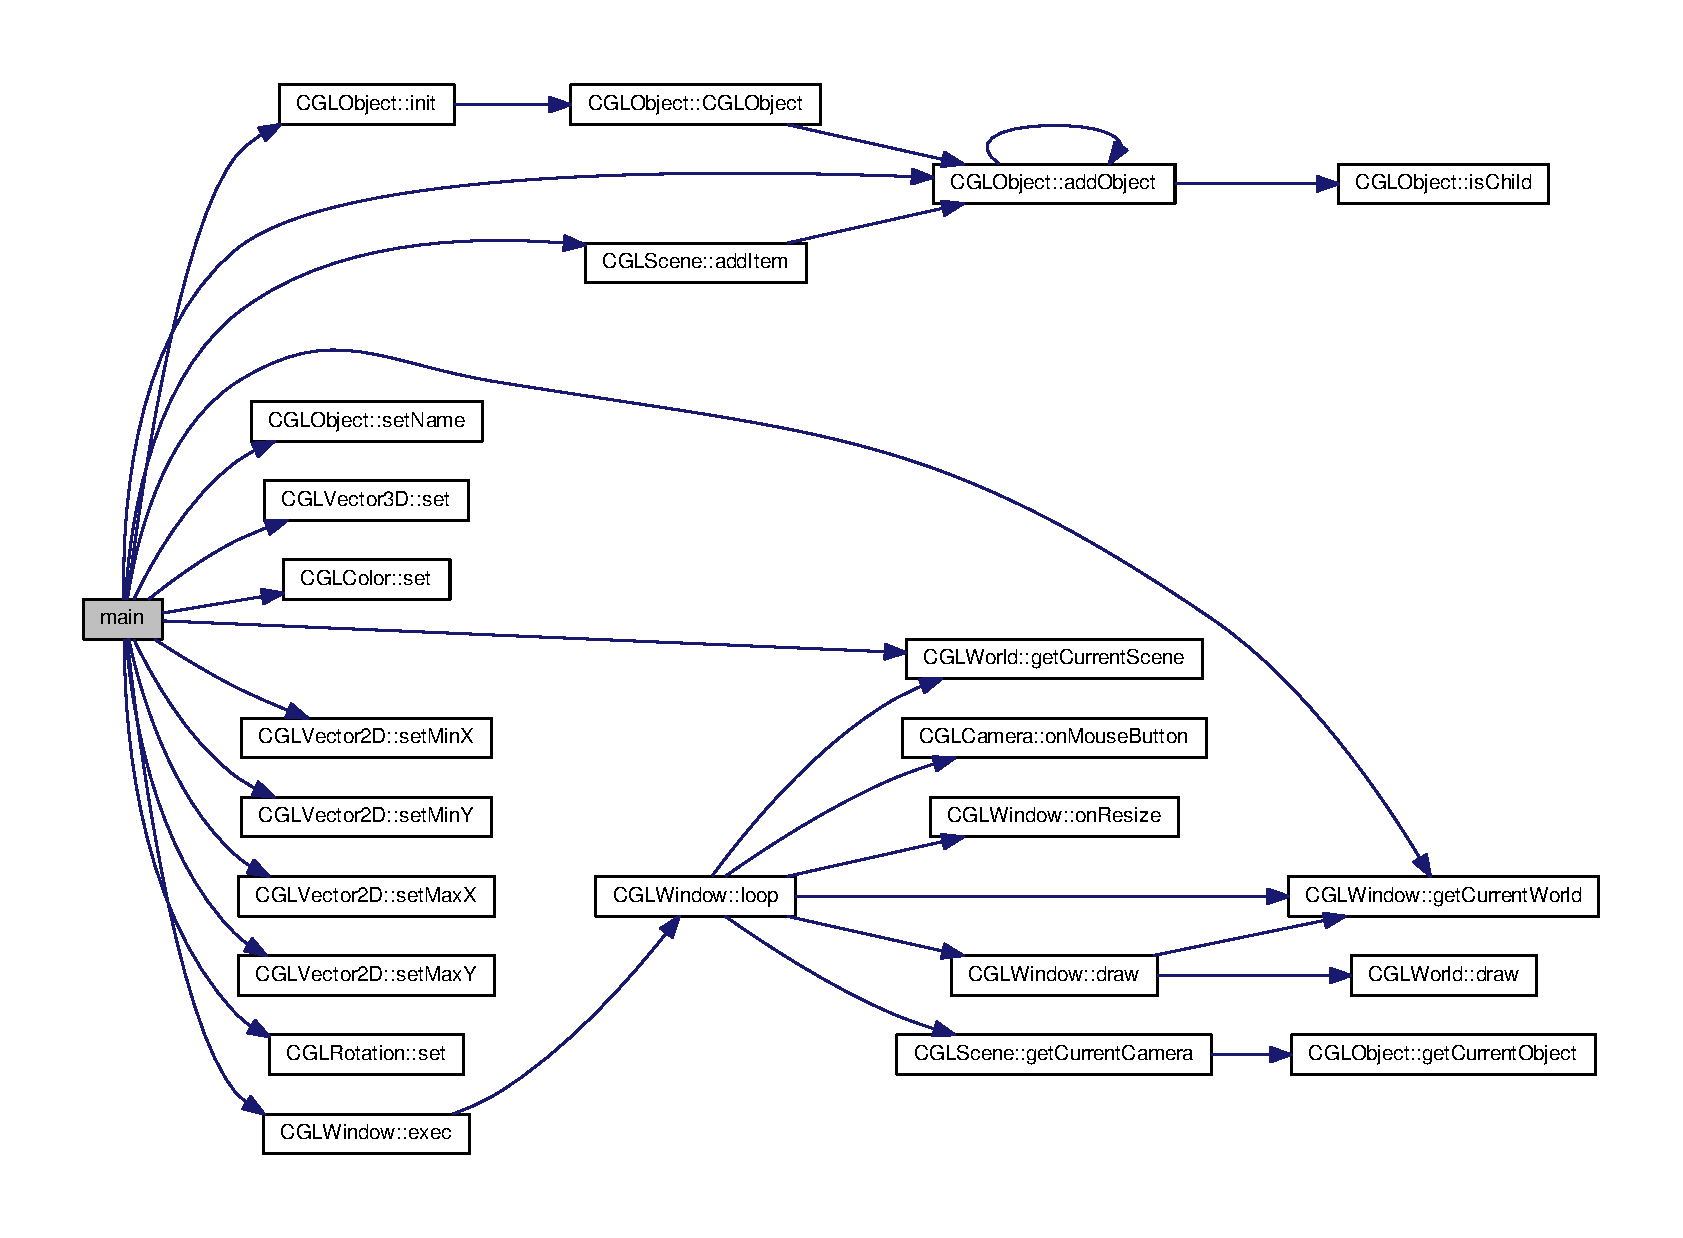
\includegraphics[width=350pt]{db/dec/_damier_g_l_8cpp_a0ddf1224851353fc92bfbff6f499fa97_cgraph}
\end{center}
\end{figure}



%--- End generated contents ---

% Index
\newpage
\phantomsection
\addcontentsline{toc}{chapter}{Index}
\printindex

\end{document}
